
\documentclass[2dCFT-lecture.tex]{subfiles}


\begin{document}


\setcounter{tocdepth}{2}

\section{Introduction}



Conformal field theories have been at the centre of much attention
during the last few decades since they are relevant for at least
three different areas of modern theoretical physics: conformal field
theories provide toy models for genuinely interacting quantum field
theories, they describe two-dimensional critical phenomena, and they
play a central role in string theory. 2d CFTs are moreover placed on mathematical rigorous footing, opening up new areas in mathematics.
Surprisingly, we can still see these trends moving forward.

In this course, we will focus on conformal field theories of \textbf{two dimensions}. However,  the subject is so rich that we can only cover the basics. To begin with, let us first introduce to conformal field theories in physics.

\subsection{Renormalization group flow and Wilson-Fisher fixed points}

In quantum field theory, a partition function is conceptually defined by using Feynmann path integral.
The basic integration variables of the path integral are the Fourier components $\phi_k$ of a field $\phi$. To impose a cutoff $\Lambda$, we schematically write
$$
\cZ= \prod_{|k|<\Lambda} \int d\phi_k\exp\left[-\cS_\Lambda[\phi_k]\right].
$$
We are interested in relating the coupling constants in a theory having energy cutoff $\Lambda$ to the coupling constants in a theory having energy cutoff $\Lambda'<\Lambda$. We redefine $\phi \rightarrow \phi+\phi'$, where $\phi'$ has non-zero Fourier modes in $\Lambda'<|k|<\Lambda$ and $\phi$ has non-zero Fourier modes in $|k|<\Lambda'$. Integrating out the field $\phi'$ gives us some result written in terms of $\phi$.
$$
\exp\left(-\cS_{\Lambda'}[\phi]\right)\ \stackrel{\mathrm{def}}{=}\  \int_{\Lambda'  \leq |k| \leq \Lambda} \mathcal{D}\phi   \exp\left[-\cS_\Lambda[\phi]\right].
$$

Whatever the result is, we include it by changing the Lagrangian to a new, \textbf{effective} Lagrangian. The explicit disappearance of the highest energy quantum modes is compensated by some change in the Lagrangian. Integrating out these modes thus has the effect of changing the coefficients of terms in the Lagrangian.  Repeatedly integrating out these thin-shells in momentum space corresponds to a smooth motion through this Lagrangian space: this is \textbf{renormalization group flow}.
\begin{figure}[ht]\centering
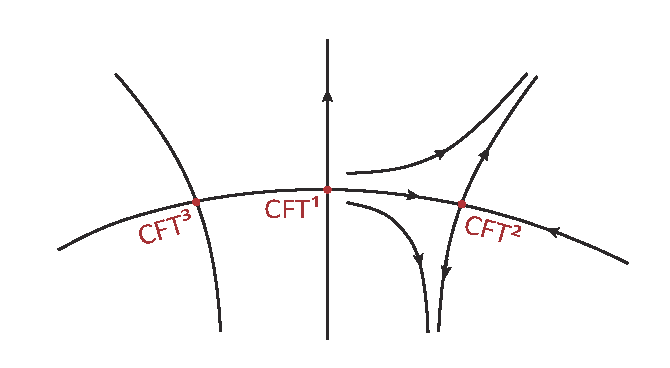
\includegraphics[width=10cm]{picture/parameter-space}
\end{figure}

By the naive dimensional analysis, the possible parameter space become finite-dimensional. Although one can consider infinitely many interaction term
$$
\cS_{int}=\int d^d x\sum g_i \mathcal{O}_i(\phi)~,
$$
the terms $\cO_i$ with $d<\Delta^i$ are suppressed at low energy, which are called \textbf{irrelevant}. Therefore, we just need to consider finitely many terms $\cO_i$ with $d\ge\Delta^i$ at low energy. To understand the behavior of a theory for these terms, we need to consider
 the beta function $\beta(g)$ describing the dependence of a coupling parameter on some energy scale $\mu$:
\begin{equation}
\beta(g)=\frac{\partial g}{\partial \log(\Lambda)}=\Lambda \frac{\partial g}{\partial \Lambda}.
\end{equation}
This implies that classical conformal invariance do not maintain conformal invariance quantum mechanically. For example, $\phi^4$ theory in $d=4$ dimensions can be shown to have the one-loop $\beta$-function
$$
\beta(\lambda)=\frac{3}{16\pi^2}\lambda^2.
$$
As we will soon see, the positive sign on this expression means the coupling constant increases with energy. These contrast with the one-loop QCD $\beta$-function,
$$
\beta(g)=-\frac{9g^3}{16\pi^2}.
$$
This $\beta$-function says the coupling decreases with energy, which is known as \textbf{asymptotic freedom}. Each of these theories, although fine classically, have length scales introduced through quantum effects. However,  if $\beta=0$,  the coupling is a constant so that the theory is scale-invariant and does not change with energy scale. The coupling constant $g^*$ with $\beta(g^*)=0$ is called \textbf{Wilson-Fischer fixed point}, and the theory at the fixed point is believed to have conformal symmetry. Therefore, conformal field theories appear at special points in the parameter spaces of quantum field theories, and they play an important role to understand families of quantum field theories.
\begin{figure}[ht]\centering
\includegraphics[width=7cm]{picture/RG}
\includegraphics[width=9cm]{picture/gapless}
\end{figure}

As we will see below, conformal field theories have more enhanced symmetries than general quantum field theories. Moreover, 2d CFTs are special because conformal symmetry becomes infinite-dimensional. In this lecture, we will study 2d CFTs by making full use of an infinite-dimensional symmetry. However, even in higher dimensions, conformal symmetries are so powerful that they provides great insights into QFTs. Moreover, if a CFT is endowed with enough supersymmetry, it is so much under control that recent study reveals some aspects of QFTs without Lagrangian description.

\subsection{Critical phenomena}

Let us recall the basics of statistical mechanics.
The partition function is defined by
$$
\mathcal{Z}=e^{-F/T}=\sum_{i} \exp \left(-\frac{\cE_i}{T} \right)
$$
where $F$ is called the free energy and and we set the Boltzmann constant $k_B=1$. Then, the probability $P_i$ that the system is in a state with energy $\cE_i$ is given by the Boltzmann distribution
$$
P_i=\frac1\cZ \exp(-\frac{\cE_i}{T})~.
$$
Therefore, the expectation value of an operator $\cO$ is given by
$$
\langle \cO \rangle=\frac{1}{\mathcal{Z}} \sum_{i}  \cO_i  ~ e^{- \cE_i / T}
$$
For instance, the average energy is
$$
E=\langle\cE\rangle=-T^2\frac{\partial}{\partial T}\left(\frac{F}{T}\right)= \frac{1}{\mathcal{Z}} \sum_{i}  \cE_i  ~ e^{- \cE_i / T}
$$

\begin{figure}[ht]\centering
\includegraphics[width=8cm]{picture/Types_of_Magnetism}
\end{figure}

Now we consider the \textbf{Ising model}  of a $d$-dimensional lattice $\Lambda$ with  $N$ lattice sites. For each lattice site $k \in \Lambda$, there is a discrete variable $\sigma_k\in  \{+1, -1\}$, representing the site's spin configuration.
The Hamiltonian of the Ising model is given by
\be\label{Ising-Hamiltonian}
\mathcal{H}=- J \sum_{\left\langle i , i^{\prime} \right\rangle} \sigma_{i} \sigma_{i^{\prime}}-B \sum_{i} \sigma_{i}
\ee
where $B$  is the external magnetic field. If $J > 0$, the alignment of spins is energetically favored and the configuration is called \textbf{ferromagnetic}. On the other hand, if $J<0$, the configuration is called \textbf{antiferromagnetic}. In the following, we will focus on the case $J>0$.


At low temperature $T$, the system settles in one of two ground states. Therefore, the magnetization $M$ has a jump discontinuity across the line of \textbf{first-order} transitions at $B=0$. A \textbf{first-order} phase transitions are the ones in which some first derivative of the free energy $F$ is discontinuous. In this example, the average energy $E$ is discontinuous.





On the other hand, the thermal fluctuations dominate at high $T$ and spins are randomly oriented (\textbf{pramagnetic}). Therefore, there is a phase transition at the critical temperature $T=T_c$ called \textbf{Curie temperature}. The magnetization is discontinuous across the phase transition, which is called the \textbf{order parameter} of the Ising model.


\begin{figure}[ht]\centering
\includegraphics[width=5cm]{picture/1st-order-PT}
\includegraphics[width=11cm]{picture/curie}
\end{figure}

To describe this critical point, we need to introduce a notion of correlation functions.  A two-point correlation function is defined as
$$
G(r)=\left\langle \sigma_{i} \sigma_{j} \right\rangle-\left\langle \sigma_{i} \right\rangle \left\langle \sigma_{j} \right\rangle \approx r^{- \tau} \mathrm{e}^{- r / \xi}
$$
where $r=|i-j|$ is the distance between the sites $i$ and $j$. In the 2d Ising model, one has $\tau =1/2$ for $T>T_c$ and $\tau =2$ for $T<T_c$.
If $r<\xi$, the two spins are correlated, since there is a large probability that they have the same value.
On the other hand, for sufficiently large $r\gg \xi$, probability should decrease roughly exponentially with $r$. Hence, the mean cluster size of correlated spins is  $\xi$, which is called the \textbf{correlation length}. As a temperature $T$ approaches $T_c$, the correlation length $\xi$ diverges, and such a critical point is called  \textbf{second-order}. At the critical point,  fluctuations on all length scales become important, and therefore the spin configuration is a fractal-like structure (Figure \ref{fig:fractal}). Consequently, the corresponding mass scale $1/\xi$ disappears and physics is described by conformal field theory at the critical point \cite[ISZ88-No.2]{Cardy:1984bb}.





\begin{figure}[ht]\centering
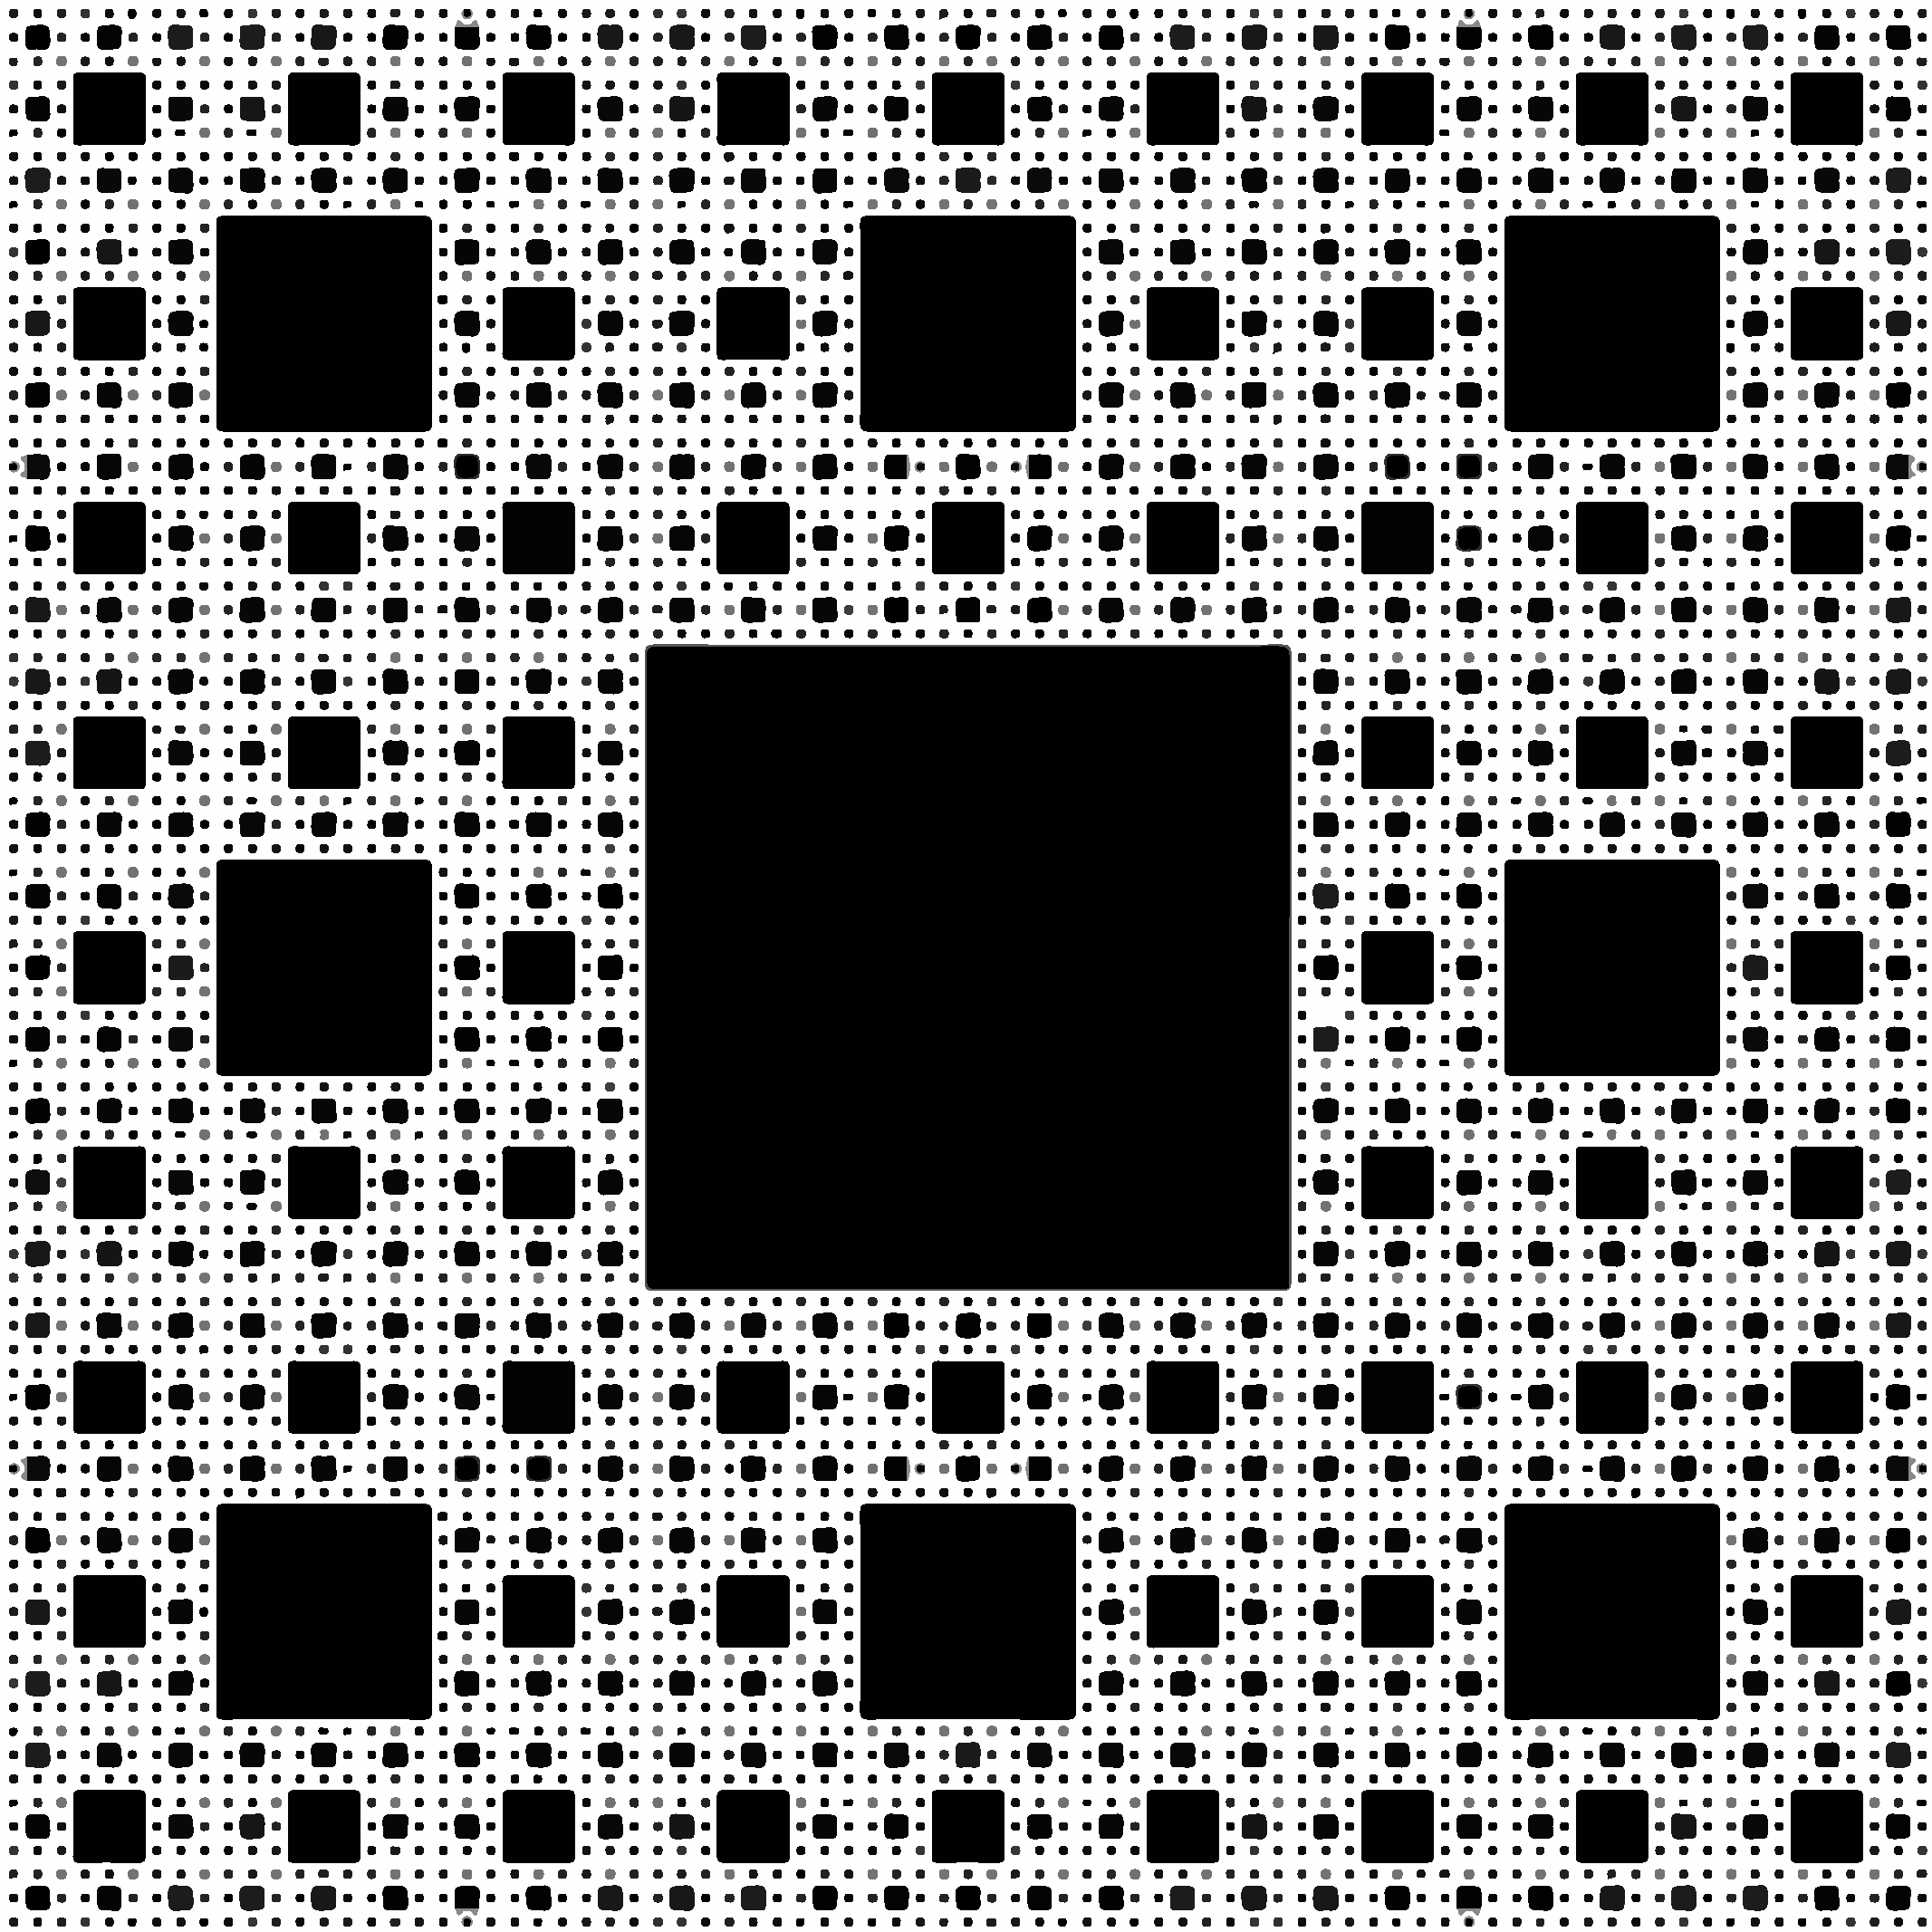
\includegraphics[width=6cm]{picture/fractal}
\caption{Schematic illustration of spin configuration at the Curie temperature $T_c$. The figure is taken from \href{https://en.wikipedia.org/wiki/Fractal}{Wikipedia:Fractal}}\label{fig:fractal}
\end{figure}


Close to the critical point, the correlation lengths and the thermodynamic quantities obey power laws, and the critical behavior near to the critical points can be  characterized by the values of the \textbf{critical exponents}.
Introducing the reduced temperature $t$ and the reduced magnetic field $h$
$$
t :=\frac{T-T_{c}}{T_{c}} \quad \text{and} \quad h :=\frac{B}{T_{c}}~,
$$
the conventional critical exponents $\a,\b,\g,\d,\nu,\eta$ are now defined by
$$
\begin{matrix}
C \sim t^{-\alpha}&(h=0)&\textrm{specific heat}\\
M \sim (-t)^\beta &(t < 0, h=0)&\textrm{spontaneous magnetization}\\
\chi \sim t^{-\gamma}&(h=0)&\textrm{zero field susceptibility}\\
M=h^{1/\delta} &(t=0)&\textrm{magnetization}\\
\xi \sim t^{-\nu}&(h=0)&\textrm{correlation length}\\
G(r) \sim  |r|^{2-d-\eta}  &(t=0,h=0)&\textrm{2pt-function}\end{matrix}
$$
where $$
C :=-\frac{T}{N} \frac{\partial^{2} F}{\partial T^{2}} , \quad M :=-\frac{1}{N} \frac{\partial F}{\partial B} \quad , \quad \chi:=\frac{\partial M}{\partial B}~.
$$
In fact, there are relations among these critical exponents and there are only two independent exponents $\nu,\eta$. In the 2d Ising model, one has
$$
\a=0~,\quad \b=\frac18~,\quad \g=\frac74~, \quad \d=15~, \quad \nu=1~, \quad \eta=\frac14
$$
Remarkably, the critical exponents stay the same even if we change the shape of lattice or we include next-nearest-neighbor interactions.
The independence of the critical exponents from such microscopic details is referred to as \textbf{universality}.

At the critical point, the two-point function can be written as
$$
\langle \sigma(x)\sigma(0)\rangle=\frac{C}{|x|^{2\Delta_\sigma}}
$$
where $\Delta_\sigma$ is called the \textbf{scaling dimension} of $\sigma$.
One can similarly define a local energy density operator
$$
\varepsilon_{i}=\sum_{i^{\prime}} J \left(i , i^{\prime} \right) \sigma_{i} \sigma_{i^{\prime}}~.
$$
Then, in the 2d Ising model, their scaling dimensions are
\be\label{Ising-conf-dim}\Delta_\sigma =1/8~,\qquad \Delta_\e: =1~,\ee
which we will see in the subsequent lectures.

\subsection{String theory}
Conformal field
theories play a central role in string theory \cite{GSW,Polchinski}. In string theory, string theory propagation on a certain manifold $M$ is described by a non-linear sigma model $\Sigma\to M$ where $\Sigma$ is a two-dimensional Riemann surface and $M$ is a certain manifold.  For instance, in a bosonic string theory, the action is expressed as
\bea\nonumber
 &\cS=\frac{1}{4\pi \alpha'} \int d^2x \left(\sqrt h h^{ab} \partial_a X^\mu \partial_b X^\nu G_{\mu\nu}(X)
 +i \varepsilon^{ab} \partial_a X^\mu \partial_b X^\nu B_{\mu\nu}(X)
 +\alpha' \sqrt h R^{(2)} \Phi(X)
 \right) \ .
\eea
where $h$ and $G$ are the metrics of $\Sigma$ and $M$, respectively, and  $B$ is an anti-symmetric field. To describe a consistent string theory, it must be a conformal
field theory. To preserve conformal invariance at quantum level, $M$ has to be 26-dimensional in bosonic string theory, and 10-dimensional in a string theory with supersymmetry. Moreover,  the vanishing one-loop renormalization group beta-functions of the non-linear sigma model implies that $M$ must be Ricci-flat.


In particular, Calabi-Yau sigma models are described by $\cN=2$ superconformal field theories. It was discovered that $\cN=2$ superconformal field theories associated to a pairs of Calabi-Yau manifolds are equivalent.
The existence of such pairs of Calabi-Yau manifolds with specified properties are known to mathematicians as the \textbf{mirror symmetry conjecture}, which is now the active subject in mathematics.

Moreover,  the equivalence between string theory on an anti-de Sitter space and conformal field theories was proposed, which is called the \textbf{AdS/CFT correspondence}. For example, this correspondence states that  non-perturbative definition of superstring theory of type IIB on AdS${}_5$ is described by the four-dimensional $\cN=4$ superconformal field theory. The AdS/CFT correspondence has been extensively studied in the last two decades, and now it has huge impact on various areas in physics.



\subsection{References}



There are too many references on 2d CFTs and each book deals with only a certain aspect of the huge subject.
In this lecture, we will first follow \cite{cardy1988conformal,ginsparg1988applied,zamolodchikov1989conformal}, and the yellow book \cite{francesco2012conformal} can be used as a dictionary. In addition,  we list some standard references related to
statistical mechanics \cite{cardy1996scaling,henkel2013conformal}, string theory \cite{Blumenhagen:2009zz,schellekens1996introduction,ketov1995conformal}, integrable systems \cite{gomez2005quantum,mussardo2010statistical}. In mathematics, studying the representation theoretic aspect of 2d CFTs has been led by Kac \cite{kac1994infinite}. Moreover, after the mathematical foundation of 2d CFTs has been given in \cite{segal1988definition} and \cite{tsuchiya1989conformal} (included in \cite{jimbo2014integrable}), 2d CFTs have shed drastically new insights in various aspects of modern mathematics
such as vertex operator algebras, moduli spaces, low-dimensional topology, geometric representation theory (for instance, see \cite{frenkel1989vertex,kohno2002conformal,frenkel2004vertex,beilinson2004chiral}). For  general conformal field theories of higher dimensions, we refer the reader to \cite{Nakayama:2013is,Qualls:2015qjb,Rychkov:2016iqz,Simmons-Duffin:2016gjk}

After this course, the reader would be highly recommended to read some of important original papers in \cite{itzykson1988conformal} so that the relevant papers in \cite{itzykson1988conformal} are indicated in this lecture note.  Related but more mathematical papers are collected in \cite{jimbo2012conformal,jimbo2014integrable}. Even in this fast-moving community, the importance of reading the classics cannot be overemphasized.

\section{Conformal invariance}

\subsection{Conformal Transformation}

A conformal transformation
is generally defined as follows:
Let us consider differentiable map
$\phi : U \rightarrow V$,
where $U$ and $V$
are  open subsets of
$M$ and $M'$ respectively.
Denoting $g$ and $g'$ as the metric tensors of
$M$ and $M'$ respectively,
we can pull back $g'$ by using the map $\phi$,
as we have learnt in differential geometry.
A conformal transformation
is then defined by such a map
that its pull back metric
$\phi^{*} g'$
satisfying the following condition:
\begin{equation}
  \phi^{*}g'=\Lambda g \, .
\end{equation}
Denoting
$x'=\phi(x)$
with $x \in U$,
we can express the condition in a covariant form:
\begin{equation}
\label{general-def-ct}
g'_{\rho\sigma}(x')
\pdv{x'^{\rho}}{x^\mu}
\pdv{x'^\sigma}{x^\nu}
=
\Lambda(x)g_{\mu\nu}(x)
\,,
\end{equation}
where $\Lambda(x)$ is a positive scalar
called the scale factor.
We see an appreciable extrapolation
from \eqref{general-def-ct},
that any smooth transformation in one dimension
is a conformal transformation.
In addition, by using
\eqref{general-def-ct},
the inner product of two arbitrary vectors $V'^{\mu}_{1}(x')$
and $V'^{\mu}_{2}(x')$
at the same point of $M'$
has a scaling effect
after its pulling back
by the conformal map:
\begin{equation}
  \label{inner-product-relation}
  g_{\mu\nu}(x)V_1^\mu(x)V_2^\nu(x)
  =
  g'_{\mu\nu}(x')V'^\mu_1(x')V'^\nu_2(x')
  \Lambda
  \, ,
\end{equation}
where $V^{\mu}_{1}(x)$
and $V^{\mu}_{2}(x)$
are the pull-back vectors respectively.
From \eqref{inner-product-relation},
it is not difficult to find that
the included angle
of two vectors
of $M'$ remains the same
when they are pulled back
by a conformal map to $M$.

In this lecture note, we focus on
$M'=M$, which implies g'=g.
We also consider $M$ to be flat spaces
with a constant metric
$\eta_{\mu\nu}
=
\text{diag}(-1,\dots,+1,\dots)$.
Thus, the condition for
a conformal transformation
can be written as
\begin{equation}
\label{def-flat-ct}
\eta_{\rho\sigma}
\pdv{x'^\rho}{x^\mu}
\pdv{x'^\sigma}{x^\nu}
=
\Lambda(x)\eta_{\mu\nu}
\, .
\end{equation}
The line element transforms
under conformal transformation as
\begin{equation}
  \dd s^2
  =
  \eta_{\mu\nu}
  \dd x^\mu \dd x^\nu
  \rightarrow
  \eta_{\rho\sigma}
  \dd x'^\rho \dd x'^\sigma
  =
  \eta_{\rho\sigma}
  \pdv{x'^\rho}{x^\mu}
  \pdv{x'^\sigma}{x^\nu}
  \dd x^\mu \dd x^\nu
  =\Lambda(x)\dd s^2
  \, .
\end{equation}
Two remarks should be stated here.
First of all,
using \eqref{def-flat-ct},
we can see
the composition of
two conformal transformation
is still conformal,
which may imply that
conformal transformations form
a group.
Secondly,
the scale factor
$\Lambda(x)=1$
corresponds to the Poincare group.

\subsection{Conditions for Conformal Invariance}
In this part, we need to figure out
some basic conformal transformations
in flat space. To begin with,
we study the infinitesimal transformations
\begin{equation}
 x'^\rho=x^\rho+\e^\rho(x)+O(\e^2)
 \, ,
\end{equation}
with an infinitesimal variable
$\e(x)\ll1$.
Plugging into the conformal condition
\eqref{def-flat-ct},
up to first order in $\e$,
the infinitesimal form
of conformal transformation
may be derived as:
\begin{equation}
\label{inf-constraint-K}
  \partial_{\mu}\e_\nu
  +
  \partial_{\nu}\e_\mu
  =
  K(x) \eta_{\mu\nu}
  \, ,
\end{equation}
with $K(x)=\Lambda(x)-1$,
some infinitesimal function.
However, since we want to find out
the explicit form for
$\e(x)$,
$K(x)$ need to be cancelled
in the constraint formula.
By tracing both sides of
\eqref{inf-constraint-K},
we have
\begin{equation}
  K(x)
  =
  \frac{2 \partial^{\mu}\e_\mu}
 {d}
  \, .
\end{equation}
Plugging back to
\eqref{inf-constraint-K},
we find the restriction depending on
$\e(x)$
to make the transformation conformal:
\begin{equation}
\label{inf-cft-e-condition}
  \partial_{\mu}\e_\nu
  +
  \partial_{\nu}\e_\mu
  =
  \frac{2}{d}
  (\partial\cdot\e)
  \eta_{\mu\nu}
  \, .
\end{equation}

\subsection{Some Useful Relation}

Let us derive two useful equations
for later purpose.
First of all, by taking
$\partial^{\nu}$
to both sides of
\eqref{inf-cft-e-condition},
we can obtain
\begin{equation}
  \partial_{\mu}
  (\partial\cdot\e)
  +
  \square\e_\mu
  =
  \frac{2}{d}
  \partial_{\mu}
  (\partial\cdot\e)
  \, .
\end{equation}
We then take $\partial_{\nu}$
to both sides:
\begin{equation}
\label{inf-cft-e-condition-2}
  \partial_{\mu}\partial_{\nu}
  (\partial\cdot\e)
  +
  \square
  \partial_{\nu}\e_\mu
  =
  \frac{2}{d}
  \partial_\nu\partial_{\mu}
  (\partial\cdot\e)
  \, .
\end{equation}
Interchanging
$\mu \leftrightarrow \nu$,
adding back to
\eqref{inf-cft-e-condition-2}
and using
\eqref{inf-cft-e-condition}
we get
\begin{equation}
  \label{e-useful-relation-1}
  (
   \eta_{\mu\nu}\square
   +
   (d-2)
   \partial_{\mu}\partial_{\nu}
 )
  (\partial\cdot\e)
  =
  0
  \, .
\end{equation}
Finally, tracing spacetime indices gives
\begin{equation}
  \label{e-useful-relation-2}
  (d-1)\square
  (\partial\cdot\e)
  =
  0
  \, .
\end{equation}

The second useful expression
is obtain by taking
$\partial_{\rho}$ of
\eqref{inf-cft-e-condition}
and permuting indices:
\bea
  \partial_{\rho}
  \partial_{\mu}
  \e_\nu
  +
  \partial_{\rho}
  \partial_{\nu}
  \e_\mu
  &=
  \frac{2}{d}
  \eta_{\mu\nu}
  \partial_{\rho}
  (\partial\cdot\e)
  \, ,
  \notag
  \\
  \partial_{\nu}
  \partial_{\rho}
  \e_\mu
  +
  \partial_{\mu}
  \partial_{\rho}
  \e_\nu
  &=
  \frac{2}{d}
  \eta_{\rho\mu}
  \partial_{\nu}
  (\partial\cdot\e)
  \, ,
  \notag
  \\
  \partial_{\mu}
  \partial_{\nu}
  \e_\rho
  +
  \partial_{\nu}
  \partial_{\mu}
  \e_\rho
  &=
  \frac{2}{d}
  \eta_{\nu\rho}
  \partial_{\mu}
  (\partial\cdot\e)
  \, .
  \notag
\eea
Subtracting the first line from
the sum of the last two leads to
\begin{equation}
\label{inf-cft-e-relation-3}
  2\partial_{\mu}
  \partial_{\nu}
  \e_\rho
  =
  \frac{2}{d}
  (
   -
   \eta_{\mu\nu}
   \partial_\rho
   +
   \eta_{\rho\mu}
   \partial_{\nu}
   +
   \eta_{\nu\rho}
   \partial_{\mu}
 )
  (\partial\cdot\e)
  \,
  .
\end{equation}

\subsection{Conformal Transformation in $d \geq 3$}\label{sec:conf-gen}

For the case $d=1$,
the relation
\eqref{e-useful-relation-2}
imposes no constraint to
$\e(x)$,
which accords with
what we have claimed,
that any smooth
transformation in one dimension
is conformal.
The case $d=2$
will be studied later
in detail.
In this section,
let's focus on the case
$d\geq 3 $.

According to
\eqref{e-useful-relation-2} for
$d \geq 3$, we have
$\square (\partial\cdot\e)=0$.
Substituting back to condition
\eqref{e-useful-relation-1}
gives
$
 \partial_{\mu}
 \partial_{\nu}
 (\partial\cdot\e)
 =
 0
$
,implying that
$(\partial\cdot\e)$
is at most linear in
$x^\mu$,
i.e.
$
 (\partial\cdot\e)
 =
 A+B_{\mu}x^\mu
$
.When plugging this linear expression
back to
\eqref{inf-cft-e-relation-3},
we immediately obtain that
$
 \partial_{\mu}
 \partial_{\nu}
 \e_\rho
$
equals to a constant.
This follows that
$\e_\mu$
is at most quadratic in
$ x^{\nu}$
and so we can make the ansatz:
\begin{equation}
\label{e-ansatz}
  \e_\mu
  =
  a_\mu
  +
  b_{\mu\nu} x^\nu
  +
  c_{\mu\nu\rho}x^\nu x^\rho
  \, ,
\end{equation}
where,
$ c_{\mu\nu\rho}
=
c_{\mu\rho\nu}
$.
For the infinitesimal nature of
$\e_\mu$,
all the constants:
$
 a_\mu,b_{\mu\nu},c_{\mu\rho\nu}
 \ll 1
$.

Noticing that all the terms in
\eqref{inf-cft-e-condition},
have only one derivative,
and that the conformal constraints
for these constants should be
independent of
$x^\mu$,
we can study the various terms in
\eqref{e-ansatz} separately.

The constant term $a_\mu$ in
\eqref{e-ansatz}
is not constrained by
\eqref{inf-cft-e-condition}.
It describes infinitesimal translation
$x'^\mu=x^\mu+a^\mu$,
for which the generator is
the momentum operator
$P_\mu=-i\partial_{\mu}$
\footnote{
	All the generators of this form can be calculated by the definition :
	\begin{equation}
	  \label{def-generator}
	  iG_a\Phi
	  =
	  \frac
	 {\delta x^\mu}
	 {\delta \omega_a}
	  \partial_{\mu}
	  \Phi
	  \, ,
	\end{equation}
	if we suppose that the fields are not affected by the transformation with $\omega_a$ the corresponding parameter.
}.

Inserting the linear term into
\eqref{inf-cft-e-condition}
, we find
\begin{equation}
\label{linear-condition}
  b_{\mu\nu}
  +
  b_{\nu\mu}
  =
  \frac{2}{d}
  (
   \eta^{\rho\sigma}
   b_{\sigma\rho}
 )
  \eta_{\mu\nu}
  \, .
\end{equation}
We then split $b_{\mu\nu}$ into
symmetric and antisymmetric part, i.e.
$b_{\mu\nu}=n_{\mu\nu}+m_{\mu\nu}$,
with
$n_{\mu\nu}=n_{\nu\mu}$
and
$m_{\mu\nu}=-m_{\nu\nu}$.
The antisymmetric part
$m_{\mu\nu}$
satisfy
\eqref{linear-condition}
automatically, while
the symmetric part gives constraint:
$
 n_{\mu\nu}
 =
 \frac{1}{d}
 (
  \eta^{\rho\sigma}
  n_{\sigma\rho}
)
 \eta_{\mu\nu}
$
, telling that the symmetric part
should be diagonal.
Therefore, we can split
$b_{\mu\nu}$ as
\begin{equation}
	b_{\mu\nu}
	=
	\alpha\eta_{\mu\nu}
	+
	m_{\mu\nu}
	\, .
\end{equation}
The symmetric term
$\alpha\eta_{\mu\nu}$
describes infinitesimal
scale transformation
$
 x'^\mu
 =
 (1+\alpha)x^\mu
$
with generator
$
  D= -ix^\mu\partial_\mu
$.
The antisymmetric part
$m_{\mu\nu} $
corresponds to infinitesimal
rotations
$
  x'^\mu
  =
  (
   \delta^\mu_\nu
   +
  {m^\mu}_\nu
 )
  x^\nu
$
with generator being the
angular momentum operator
$
  L_{\mu\nu}
  =
  i(
  x_\mu\partial_\nu
  -
  x_\nu\partial_\mu
 )
$.


Now let us consider the quadratic term.
By inserting the quadratic term into
\eqref{inf-cft-e-relation-3}, after straight-forward calculation,
we find that
\begin{equation}
  c_{\mu\nu\rho}
  =
  \eta_{\rho\mu}f_\nu
  +
  \eta_{\mu\nu}f_\rho
  -
  \eta_{\nu\rho}f_\mu
  \, ,
\end{equation}
with
$f_\mu=\frac{1}{d}{c^\rho}_{\rho\mu}$.
The resulting transformations are
\begin{equation}
\label{inf-SCT}
  x'^\mu
 =
  x^\mu
  +
  2(x\cdot f)x^\mu
  -(x\cdot x)f^\mu
  \, ,
\end{equation}
which are called
\textbf{special conformal transformations}
(SCT)
and the corresponding generator is
$
 K_\mu
=
 -i(
     2 x_\mu x^\nu\partial_\nu
     -
     (x\cdot x)\partial_{\mu}
)
$
.

\subsection{Finite Conformal Transformation}
So far, we have identified
all basic infinitesimal conformal transformations
and their generators.
However, in order to determine
the conformal group,
we also need the corresponding
finite transformations.
All the basic
finite conformal transformations
are shown in Table \ref{Tab:fin-ct}.
\begin{table}[htbp]
	\centering
	 \caption{Finite conformal transformations
	 and corresponding generators}
	 \label{tab:ModelASymbol}
	 \begin{tabular}{lll}
	 	\toprule
	 	  Transformations
	 	&
	 	& Generators
	 	\\
	 	\midrule
	 	  translation
	 	& $x'^\mu=x^\mu+a^\mu$
	 	& $P_\mu=-i \partial_\mu$
	 	\\
	 	  dilation
	 	& $x'^\mu= \alpha x^\mu$
	 	& $D=-ix^\mu
	 	   \partial_\mu
	 	  $
	 	\\
	 	  rotation
	 	& $x'^\mu
	 	   ={M^\mu}_\nu x^\nu
	 	  $
	 	& $L_{\mu\nu}=
	 	   i(
	 	   x_\mu\partial_\nu
	 	   -
	 	   x_\nu\partial_\mu
	 	  )
	 	  $
	 	\\
	 	  SCT
	 	& $x'^{\mu}=
	 	   \frac
	 	  {x^\mu-(x\cdot x)f^\mu}
	 	  {
	 	   	1-2(f\cdot x)
	 	   	+
	 	   	(f\cdot f)(x\cdot x)}
	 	  $
	 	& $K_\mu=-i(
	 	   2 x_\mu x^\nu\partial_{\nu}
	 	   -
	 	   (x\cdot x)\partial_\mu
	 	  )
	 	  $
	 	\\
	 	\bottomrule
	 \end{tabular}\label{Tab:fin-ct}
\end{table}
The finite transformations
for translation and rotation
are Poincare transformations
we are familiar with.
The finite transformation for
dilation can be derived from
it infinitesimal  form easily.
Thus, what we focus on is
the finite transformation
for SCT.
It is hopeless to derive it
through its infinitesimal form.
But, we can guess this finite
form of transformation,
if we realize that an inversion
$x'^\mu=\frac{x^\mu}{x\cdot x}$
is also a conformal map. By plugging
in to \eqref{def-flat-ct},
we can obtain its scale factor as
$\Lambda(x)=(x\cdot x)^{-2}$.
Inversion can be one of the
basic finite conformal transformation
instead of SCT.
However, it has neither
infinitesimal form nor parameters.
Now we want to
construct finite SCT.
Using the transitive property
for conformal map,
we can thus first make
an inversion of
$x^\mu$, then
make an translation
$f^\mu$,
and inverse the result again
to construct a new
conformal transformation.
An illustration in two dimensions
is shown in
Figure \ref*{fig:SCT-ill}.
As $f^\mu$ goes to zero,
$x^\mu$ maps to itself.
Therefore it should have
infinitesimal form.
\begin{figure}[ht]
	\centering
	\includegraphics
	[width=0.7\linewidth]
	{picture/SCT-ill.pdf}
	\caption
	{
		Illustration of a finite
		Special Conformal
		Transformation
	}
	\label{fig:SCT-ill}
\end{figure}
\begin{equation}
\label{fin-SCT}
  x'^\mu
 =\frac
   {
      \frac{x^\mu}{x\cdot x}
      -f^\mu
  }
   {
      (\frac{x^\mu}{x\cdot x}
      -f^\mu)
      (\frac{x^\mu}{x\cdot x}
      -f^\mu)
  }
 =\frac
   {x^\mu-(x\cdot x)f^\mu}
   {
  	 1-2(f\cdot x)
  	 +
  	 (f\cdot f)(x\cdot x)
  }
    \, .
\end{equation}
The result is what we have shown in
Table \ref{Tab:fin-ct}.
It is easy to verify that
when $f^\mu \rightarrow 0$,
\eqref{fin-SCT} reduces to
infinitesimal form of SCT:
\eqref{inf-SCT}.
Further more
by using
\eqref{def-flat-ct},
after a heavy and tedious calculation,
the scale factor for SCT
can be computed as
\begin{equation}
  \Lambda(x)
  =
  (1-2(f\cdot x)+ (f\cdot f)(x\cdot x))^{-2}
\end{equation}
Finally, we observe from
\eqref{fin-SCT},
that
the finite SCT are not globally defined.
In particular,
for a given non-zero vector
$f^\mu$,
there is a point
$x^\mu=\frac{1}{f\cdot f}f^\mu$
such that
$x^\mu$
is mapped to infinity.
(The denominator goes to
 zero more quickly
 than the numerator.)
Therefore, in order to define
the arbitrary conformal transformation, the point at infinity should
be included.

\subsection{Conformal Groups and Algebras}

The conformal transformations form a group, called the conformal group of dimension $d\ge3$.
Actually,
the algebra generated by
infinitesimal conformal transformations
is the Lie algebra of the conformal group, called the
conformal algebra.

Let us identify the conformal algebra  of dimension $d\ge3$.
The dimension of the algebra is
$N=d+1
  +\frac{d(d-1)}{2}
  +d
  =\frac{(d+2)(d+1)}{2}
$
by counting the generators in
Table \ref{Tab:fin-ct}.
The commutation rules
with no central charge
can be obtained
by direct calculations.
\bea
\label{com-rela-conf}
   \comm{D}{P_\mu}
   &=
   i P_\mu
   \notag\, ,\\
   \comm{D}{K_\mu}
   &=
   -i K_\mu
   \notag\, ,\\
   \comm{K_\mu}{P_\nu}
   &=
   2i(
   \eta_{\mu\nu}D
   -
   L_{\mu\nu}
  )
   \notag\, ,\\
   \comm{K_\rho}{L_{\mu\nu}}
   &=
   i(
   \eta_{\rho\mu}K_\nu
   -
   \eta_{\rho\nu}K_\mu
  )
   \, ,\\
   \comm{P_\rho}{L_{\mu\nu}}
   &=
   i(
   \eta_{\rho\mu}P_\nu
   -
   \eta_{\rho\nu}P_\mu
  )
   \notag\, ,\\
   \comm{L_{\mu\nu}}{L_{\rho\sigma}}
   &=
   i(
   \eta_{\rho\nu}L_{\mu\sigma}
   +
   \eta_{\mu\sigma}L_{\nu\rho}
   -
   \eta_{\rho\mu}L_{\nu\sigma}
   -
   \eta_{\nu\sigma}L_{\mu\rho}
  )
   \notag\, .
\eea
To put the above commutation relations
into a simpler form,
we define the following generators.
\bea
   &J_{\ \mu,\nu}
   =
   L_{\mu,\nu}
   \, ,\notag \\
   &J_{-1,0}
   =
   D
   \, ,\notag \\
   &J_{-1,\mu}
   =
   \frac{1}{2}
   (P_\mu-K_\mu)
   \, ,\\
   &J_{\ 0,\mu}
   =
   \frac{1}{2}
   (P_\mu+K_\mu)
   \, .\notag
\eea
By using
\eqref{com-rela-conf},
we can verify that
$J_{m,n}$ with
$m,n=-1,0,1,\dots d$,
satisfy the following commutation relations:
\begin{equation}
\label{simper-conf-algebra}
  \comm{J_{mn}}{J_{rs}}
  =
  i(
  \eta_{ms}J_{nr}
  +
  \eta_{nr}J_{ms}
  -
  \eta_{ms}J_{ns}
  -
  \eta_{ns}J_{mr}
 )
  \, .
\end{equation}
For Euclidean $d$-dimensional
space $\mathbb{R}^{d}$, we see
the metric
$\eta_{mn}$ here
is
$\eta_{mn} =$
$\text{diag}(-1,1,\dots,1)$ so that
we identify
\eqref{simper-conf-algebra}
with the commutation relations
of the Lie algebra
$\mathfrak{so}(1,d+1)$.
We can generalize the result
to the space $\mathbb{R}^{p,q}$,
with
$d=p+q \geq 3$.
The corresponding conformal group
is
$SO(p+1,q+1)$.



\subsection{2d Conformal Transformation}\label{sec:2d-conf-trans}
In this section, we will focus on the
special case of two dimensions with
Euclidean metric.
From \eqref{inf-cft-e-condition}, the infinitesimal condition for
conformal transformation
in two dimensions
reads as follows:
\begin{equation}
\label{C-R equation}
  \partial_1\e_1
  =
  \partial_2\e_2
  \, ,
  \qquad
  \partial_1\e_2
  =
  -\partial_2\e_1
  \, .
\end{equation}
\eqref{C-R equation}
tells us that
if we introduce complex variables :
\bea
\label{coordinate transformation}
  z= x^1+i x^2
  \,  ,\qquad
  \e=\e^1+i \e^2
  \,  ,\notag \\
  \overline{z}= x^1-ix^2
  \,  ,\qquad
  \overline{\e}= \e^1-i \e^2
  \, ,
\eea
according to
Cauchy-Riemann equations
in complex analysis,
$\e(z)$ is a holomorphic function
(in some open set).
Equivalently any infinitesimal
holomorphic transformation
$z'=z+ \e(z)$
gives rise to a
two-dimensional conformal transformation.

In fact, any holomorphic function on
the complex plane
is conformal
(i.e, preserves angles).
To prove this,
we should rewrite
the definition of
a conformal transformation
\eqref{def-flat-ct}
with complex variables.
Let us first, rewrite the line element:
\begin{equation}
  ds^2=(\dd x^1)^2+(\dd x^2)^2
      =\dd z \dd \overline{z}
      =g_{\alpha\beta}z^\alpha z^\beta
      \, ,
\end{equation}
with $z^1=z$, $z^2=\overline{z}$.
The flat space metric
in complex coordinates
can be obtained:
\begin{equation}
\label{metric-complex-space}
  g_{\alpha\beta}
  =
  \mqty(
       0 & \frac{1}{2}\\
       \frac{1}{2} & 0
      )
  \, ,
  \qquad
  g^{\alpha\beta}
  =
  \mqty(
       0 & 2 \\
       2 & 0
      )
  \, .
\end{equation}
The condition
\eqref{def-flat-ct}
now becomes:
\begin{equation}
  \label{def-flat-ct-complex}
  g_{\alpha\beta}
  \pdv{z'^\alpha}{z^\gamma}
  \pdv{z'^\beta}{z^\delta}
  =
  \Lambda(z,\overline{z})g_{\gamma\delta}
  \, ,
\end{equation}
which is satisfied,
if $z'=f(z)$
is a holomorphic function.
The conformal factor is then
$\Lambda(z,\overline{z})
=
\abs{\pdv{f(z)}{z}}^2$.
Figure \ref{fig:2dcft-ill}
shows some examples on
conformal transformations.
We can see that an angle at any point is preserved when
$z'=f(z)$ is holomorphic.
\begin{figure}[ht]
	\centering
	\caption{Coordinate transformation:
		The transformation from
		square lattice (a),
		onto the lattice in (b) and (c)
		is conformal,
		while the transformation
		onto the lattice in (d) is not.}
	\label{fig:2dcft-ill}
	\subfigure[$z$]{
	\includegraphics[width=0.3\textwidth]{picture/2dcft-1}}
    \subfigure[$z'=z^2$]{
	\includegraphics[width=0.3\textwidth]{picture/2dcft-2}}
    \subfigure[$z'=1/z$]{
	\includegraphics[width=0.3\textwidth]{picture/2dcft-3}}
    \subfigure[$z'=z\abs{z}$]{
    \includegraphics[width=0.3\textwidth]{picture/2dcft-4}}
\end{figure}

\subsubsection*{Witt algebra}

As we have seen above,
for an infinitesimal conformal
transformation in two dimensions,
$\e(z)$ has to be holomorphic in
some open set.
We can locally around say
$z=0$
perform a Laurent expansion of
$\e(z)$.
A general infinitesimal conformal
transformation thus can be written as
\bea
\label{2d-inf-Laurant}
  z'&=z+\e(z)
     =z
    +\sum_{n\in\mathbb{Z}}
     \e_n(-z^{n+1})
     \notag \, , \\
  \overline{z}' &=z+ \overline{\e}(\overline{z})
     =\overline{z}
    + \sum_{n\in\mathbb{Z}}
     \overline{\e}_n
     (-\overline{z}^{n+1})
     \, ,
\eea
where $\e_n$ and $\overline{\e}_n$ are
infinitesimal parameters.
Supposing a spinless and dimensionless
field $\phi(z,\overline{z})$
living on the plane,
the effect of such a mapping would be:
\begin{equation}
  \label{tran-scalar-field}
  \phi(z,\overline{z})
  \rightarrow
  \phi'(z',\overline{z}')
  =
  \phi(z,\overline{z})
  \, ,
\end{equation}
or
\bea
  \delta{\phi}
  &\equiv
  \phi'(z,\overline{z})
  -\phi(z,\overline{z})
  =\phi'(z'-\e(z),\overline{z}'-\bar\e(\overline{z}))
  -\phi(z,\overline{z})
  \notag\\
  &=
  -\e(z)\partial\phi
  -\bar\e(\overline{z})\overline{\partial}\phi
  +o(\e)
  =
  -\sum_{n\in\mathbb{Z}}
  (\e_n l_n \phi(z,\overline{z})
   +
   \bar\e_n \overline{l}_n \phi(z,\overline{z})
 )
  \, ,
\eea
where we have introduced the generators
\begin{equation}
l_n=- z^{n+1}\partial\,,
\qquad
\overline{l}_n=-\overline{z}^{n+1} \bar\partial
\, .
\end{equation}
We find the number of
independent infinitesimal conformal transformations is infinite.
The commutators for these
local generators can be calculated straightforward then:
\bea
\label{Witt-algebra}
  \comm{l_n}{l_m}
  &=
  (m-n) l_{n+m}
  \, ,\notag \\
  \comm{\overline{l}_m}{\overline{l}_n}
  &=
  (m-n)\overline{l}_{m+n}
  \, , \\
  \comm{l_m}{\overline{l}_n}
  &=0
  \, .\notag
\eea
The first commutation
relations define one copy of the
so-called Witt algebra.
We can observe that the local
conformal algebra
\eqref{Witt-algebra}
is the direct sum of two
Witt algebras.

\subsubsection*{M\"obius transformation}
A global conformal transformation
in two dimensions
is defined to be invertible
and well-defined on the
Riemann sphere
$S^2 \simeq \mathbb{C}\cup
\{\infty\}$.
Thus, it should be generated
by the global-defined
infinitesimal generators.
At $z=0$, we find that
$l_n=- z^{n+1}\partial_z$,
is non-singular only for
$n\geq-1$.
At $z=\infty$,
let us perform the change
of variable
$z=-\frac{1}{w}$,
and study $w \rightarrow 0$.
We then observe that
$l_n=-(-\frac{1}{w})^{n-1}\partial_w$,
is nonsingular at
$w=0$ only for
$n\leq 1$.
Therefore, globally defined
conformal transformations
on the Riemann sphere
$S^2=\mathbb{C}\cup\{\infty\}$
are generated by
$\{l_{-1},l_0,l_{+1} \}$.
Through the Wit algebra
\eqref{Witt-algebra},
we immediately see that these three
generators form a close subalgebra
of Wit algebra,
which implies
the corresponding conformal transformations
form a globally defined group,
called the conformal group
in two dimensions.
The discussion of
antiholomorphic counterpart
is similar.

Now, we are going to study
the conformal group in two dimensions
deeply.
From the Laurent expansion
\eqref{2d-inf-Laurant},
the operator
$l_{-1}= -\partial_z$, generates
the infinitesimal transformation
$z'=z-\e_{-1}$.
Thus, $l_{-1}$ is the
generator of translations
$z\mapsto z+b$ with $b$
an arbitrary complex constant.

For $n=0$, the operator
$l_0=-z\partial_z$,
generates the linear term of
\eqref{2d-inf-Laurant}.
It is not difficult to verify that
the corresponding finite transformation is
$z'=a z$, with $a$
an arbitrary complex constant.
The modulus of $a$
turns out to lead a dilatation,
while the phase of $a$ gives rise to
a rotation.
In order to get a geometric intuition of
such transformations, we can perform the
change of variables $z=r e^{i\phi}$ to find
\begin{equation}
  l_0=-\frac{1}{2} r \partial_r
       +\frac{i}{2}\partial_\phi\, ,
  \qquad
  \overline{l}_0=- \frac{1}{2}r \partial_{r}
       -\partial_\phi \, .
\end{equation}
We can perform the linear combinations
\begin{equation}
  \label{l0combinations}
  l_0+\overline{l}_0=- r \partial_r\, ,
  \qquad
  i(l_0-\overline{l}_0)=-\partial_\phi\, .
\end{equation}
Therefore, we see that $l_0+\overline{l}_0$ is the
generator for two-dimensional dilations and
that $i(l_0-\overline{l}_0)$ is the generator of
rotations.

Finally, the operator $l_{+1}$
generates the infinitesimal quadratic term.
By the variable changing
$w=-\frac{1}{\cZ}$,
the operator turns out to be
$l_{+1}=-\partial_w$,
which corresponds to a translation of $w$:
$w\mapsto w-c$.
Therefore, the operator $l_{+1}$ generates
Special Conformal Transformations:
$z\mapsto \frac{z}{cz+1}$.

The complete set of mappings discussed
above is of the form
\begin{equation}
  z\mapsto \frac{a z+b}{cz+d}
  \, ,
\end{equation}
with $a,b,c,d \in \mathbb{C} $.
For this transformation
to be invertible, we have to require
that $ad-bc \neq 0$.
If this is the case, we can
scale the constants $a,b,c,d$,
such that $ad-bc =1$.
Furthermore, the expression is
unaffected by taking all of
$a,b,c,d$ to minus themselves.
These mappings are called projective
transformations.
We see each global conformal transformation
in 2 dimensions can be associated
with a matrix
$\mqty(a & b \\ c & d)$.
For instance:
\bea
	&\text{translation}:\qquad
	z\mapsto z+b
	\quad
	\Leftrightarrow
	\quad
	\mqty(1 & b \\ 0 & 1)
	\, ,\notag\\
	&\text{dilatation}:\quad
	z\mapsto a z\, , a\in \mathbb{R}
	\,
	\Leftrightarrow
	\,
	\mqty(\sqrt{a} & 0\\
	      \sqrt{0} & \sqrt{1/a}
	    )
	\, ,\notag \\
	&\text{rotation}:
	\qquad
	z\mapsto e^{i\theta}\, ,
	\theta\in \mathbb{R}
	\,
	\Leftrightarrow
	\,
	\mqty(e^{i\theta/2} & 0\\
	      0 & e^{-i\theta/2}
	    )
	\, ,\notag \\
	&SCT:
	\qquad\qquad
	z\mapsto \frac{z}{c z +1}
	\quad
	\Leftrightarrow
	\quad
	\mqty(1 & 0 \\
	      c & 1)
	 \, .\notag
\eea
We can infer that the conformal
group of the Riemann sphere
$S^2=\mathbb{C} \cup \{\infty \}$
is the  M\"obius group
$SL(2,\mathbb{C})/\mathbb{Z}_2$.










\section{Basics in Conformal Field Theory}
Conformal field theories are quantum field theories invariant under conformal transformation. In this section, we will see this simple statement results in powerful constraints in two-dimensional system.


\subsection{Noether theorem and Ward-Takahashi identity}
In this subsection, let us review
the role of symmetry in quantum field theory.

\subsubsection*{Continuous Symmetry Transformation}
In the following sections,
we focus on coordinate transformations,
while in field theory,
we still need to consider
the transformation of fields.
In the previous sections, we have used transformations of spinless field
\eqref{tran-scalar-field},
to obtain the
corresponding generators.
However, sometimes field
might have its own
non-trivial transformation rules.
Figure \ref{fig:symmetry} shows the rotation
transformation of a vector field.
We see field $\Phi$ rotates under the
coordinate transformation.
\begin{equation}
  \label{trans-field-general}
  x\rightarrow x'\, ,
  \qquad
  \Phi(x)\rightarrow\Phi'(x')
  =\mathcal{F}(\Phi(x)) \, .
\end{equation}
Functional change $\mathcal{F}$
can be obtained by studying the
representation theory of coordinate
transformation group. We will not
illustrate more on this,
but give some examples
for later use.
\begin{figure}[ht]
	\centering
	\caption{Rotation transformation of a vector field.}
	\includegraphics[width=0.5\linewidth]{picture/Symmetry}
	\label{fig:symmetry}
\end{figure}

Let us start with a rather trivial one,
a translation:
\begin{equation}
  \label{translation-field}
  x'=x+a\, ,
  \qquad
  \Phi'(x+a)=\Phi(x)\, ,
\end{equation}
which implies that functional change
$\mathcal{F}$ is trivial here.

Next, we consider a Lorentz transformation
(rigid rotation).
In general it takes the following form:
\begin{equation}
  \label{lorentz-field}
  x'^\mu ={\Lambda^\mu}_\nu x^\nu\, ,
  \qquad
  \Phi'(\Lambda x) =U(\Lambda)\Phi(x)\, ,
\end{equation}
where $U(\Lambda)$ is a transformation matrix acting on $\Phi$.\footnote{
	In quantum field theory,
	$\Phi$ is more likely to treat as an operator with transformation rule:
	\begin{equation}
	\Phi'(\Lambda x)
	=U^{-1}(\Lambda)\Phi(x)U(\Lambda)\, .
	\notag
	\end{equation}
}
The infinitesimal form of
$U(\Lambda)$ is
\begin{equation}
 \label{U-Lambda-inf}
 U(\Lambda)=1-\frac{1}{2}i
 \omega_{\rho\nu}
 S^{\rho\nu}\, ,
\end{equation}
where $\omega_{\rho\nu}$ are infinitesimal
parameters for Lorentz transformation
and $S^{\rho\nu}$ is a representation of the Lorentz algebra.

Finally, under a scale transformations,
we have
\begin{equation}
  \label{scale-field}
  x'=\lambda x \, ,
  \qquad
  \Phi'(\lambda x)=\lambda^{-\Delta}
  \Phi(x) \, ,
\end{equation}
where $\Delta$ is the scaling dimension
of the field.

\subsubsection*{Generator}
In a field theory, the generator
of a symmetry depends on
transformation of field
as well as of coordinate.
The infinitesimal form of
\eqref{trans-field-general}
can be written as:
\bea
\label{trans-field-general-inf}
  x'^{\mu} &= x^\mu+\omega_a
  \frac{\delta x^\mu}{\delta \omega_a}
  \, ,
  \notag\\
  \Phi'(x') &= \Phi(x)
  +
  \omega_a \frac{\delta\mathcal{F}}
 {\delta \omega_a}(x)
  \, .
\eea
Here $\{\omega_a\}$ is a set of
infinitesimal parameters.
Now it is customary to define
the generator $G_a$ of a
symmetry transformation by
the following expression:
\begin{equation}
\label{def-generater-general}
  \delta_\omega
  \Phi(x)
  \equiv \Phi'(x)-\Phi(x)
  \equiv
  -i\omega_a G_a \Phi(x)\, ,
\end{equation}
which is just
the infinitesimal transformation
of field at a same point.
Together with
\eqref{trans-field-general-inf},
to first order, we obtain the
explicit expression:
\begin{equation}
  \label{def-generator-general-explicit}
  iG_a \Phi
  =
  \frac{\delta x^\mu}{\delta \omega_a}
  \partial_\mu \Phi
  -
  \frac{\delta\mathcal{F}}{\delta \omega_a}
  \, .
\end{equation}
For a field satisfying $\Phi'(x')=\Phi(x)$,
the expression reduces to
\eqref{def-generator}.
Using the definition
\eqref{def-generator-general-explicit},
and combining with
the infinitesimal field of
\eqref{translation-field},
\eqref{lorentz-field} and
\eqref{scale-field}, we can write
the corresponding generators in field space
\bea
  \label{generator-three-field}
  &\text{translation}:
  \qquad  P_\nu=-i\partial_\nu \, ,
  \notag \\
  &\text{rotation} :
  \qquad L^{\rho\nu}
  =i(x^\rho\partial^\nu
  -x^\nu\partial^\rho)
  +S^{\rho\nu}
  \, ,\\
  &\text{dilatation}:
  \qquad
  D=-i x^\nu \partial_\nu
  -i\Delta
  \, . \notag
\eea
We see that when field transformation
$\mathcal{F}(\Phi)$ is trivial,
three expressions in
\eqref{generator-three-field} reduce
to the first three generators in
Table \ref{tab:ModelASymbol}.

\subsubsection*{Noether's Theorem}
We now derive Noether's theorem,
which states that to every continuous
symmetry of the action one may associate
a conserved current at classical level.
Let us consider an action in $d$ dimensions
\begin{equation}
 \cS=\int \dd^d x
 \mathcal{L}(\Phi,\partial_\mu \Phi)
\end{equation}
which is endowed with symmetry generated by $\omega_aG_a$.
Under the continuous
transformation
\eqref{trans-field-general},
the action becomes
\bea
  \cS' &= \int \dd^d x'
  \mathcal{L}(
  \Phi'(x'),\partial_\mu'\Phi'(x'))
  \notag\\
  &=\int \dd^d x \abs{\pdv{x'}{x}}
  \mathcal{L}
  (\mathcal{F}(\Phi(x)),(\pdv{x^\nu}{x'^\mu})
  \partial_\nu \mathcal{F}(\Phi(x)))\, .
\eea
Using the infinitesimal form for transformation
\eqref{trans-field-general-inf},
we get
\bea
\cS'=\int \dd^d x \bigg(1+\partial_\mu
     (\omega_a \frac{\delta x^\mu}
    {\delta \omega_a})\bigg)
     \mathcal{L}
     \Bigg(
     \Phi+\omega_a
     \frac{\delta\mathcal{F}}
    {\delta\omega_a},
     \bigg(
     \delta^\nu_\mu
     -
     \partial_\mu
     (
     \omega_a\frac{\delta x^\nu}
    {\delta \omega_a}
    )
     \bigg)
     \bigg(
     \partial_\nu \Phi+
     \partial_\nu
     (
     \omega_a\frac{\delta\mathcal{F}}
    {\delta\omega_a}
    )
     \bigg)
    \Bigg)\, .
\eea
Since $\omega_aG_a$ is symmetry of the action, $\delta \cS=\cS'-\cS$  vanishes if $\omega_a$ is a constant.
Thus, the contribution from all terms with no derivatives
of $\omega_a$ in the variation must be zero.
Therefore, to first order, the variation
involves only the first derivatives of
$\omega_a$, obtained by expanding the
Lagrangian so that we can write
\begin{equation}
   \delta \cS=- \int \dd^d x ~
   j^\mu_a \partial_\mu \omega_a\, ,
\end{equation}
where $j^\mu_a$ is called the current
associated with the infinitesimal transformation:
\begin{equation}
  \label{cano-current}
  j^\mu_a =\bigg(
  \pdv{\mathcal{L}}{
   (\partial_\mu\Phi)}
   \partial_\nu \Phi
  -
   \delta^\mu_\nu
   \mathcal{L}
  \bigg)
  \frac{\delta x^\nu}{\delta\omega_a}
  -
  \pdv{\mathcal{L}}{(\partial_\mu \Phi)}
  \frac{\delta\mathcal{F}}{\delta\omega_a}
  \, .
\end{equation}
The integral by parts yields
\begin{equation}
  \label{variation-action-locally}
  \delta \cS=\int \dd^d x \,\omega_a \partial_\mu
  j^\mu_a
  \, .
\end{equation}
If the field configurations satisfy the
classical equations of motion,
the action is invariant under any
variation of the fields. Thus
$\delta \cS$ should vanish for any parameters
$\omega_a(x)$. This implies the
conservation law:
\begin{equation}
\partial_\mu j^\mu_a=0 \, .
\end{equation}
The associated  charge
\begin{equation}
\label{def-conserved-charge}
  Q_a=\int \dd^{d-1} x \, j^0_a \, ,
\end{equation}
is conserved because its time derivative vanishes
\begin{equation}
  \frac{d}{dt}{Q}_a=\int \dd^{d-1} x ~
  \partial_0 j_a^0
  =-\int \dd^{d-1}x ~ \partial_i j^i
  =0\, .
\end{equation}
One remark  to be mentioned here
is that we may freely add to the expression
\eqref{cano-current}
the divergence of
an antisymmetric tensor without
affecting the conservation law:
\begin{equation}
  \label{current-freedom}
  j^\mu_a \rightarrow
  j^\mu_a +\partial_\nu B^{\nu\mu}_a
  \, ,
  \qquad
  B^{\nu\mu}_a=- B^{\mu\nu}_a
  \, .
\end{equation}

Let us now focus on an important example. First of all,
if the action is invariant under translation
$x'^\mu\rightarrow x^\mu +\e^\mu$,
we can associate it with a current by using
\eqref{cano-current}:
\begin{equation}
  \label{cano-ener-mon-tensor}
  T^{\mu\nu}_{\text{c}}=
  -\eta^{\mu\nu}\mathcal{L}
  +\pdv{\mathcal{L}}{(\partial_\mu\Phi)}
  \partial^\nu \Phi \, ,
\end{equation}
which is the \textbf{energy-momentum
tensor}.
However, the canonical energy-momentum
tensor $T^{\mu\nu}_\text{c}$ is generally not
symmetric under $\mu$ and $\nu$. However, we have freedom to
modify this tensor as illustrated
in \eqref{current-freedom},
to make it
symmetric.
\begin{equation}
  \label{freedom-energy-momentum-tensor}
  T^{\mu\nu}_{\text{B}}=
  	T^{\mu\nu}_\text{c}
  	+\partial_\rho B^{\rho\mu\nu}\,
  	,\quad
  	B^{\rho\mu\nu}=-B^{\mu\rho\nu}\, .
\end{equation}

Now consider the conserved current
associated with Lorentz transformation.
By using the infinitesimal form
\eqref{U-Lambda-inf}, the conserved
current becomes
\begin{equation}
  j^{\mu\nu\rho}=
  T^{\mu\nu}_{\text{c}}x^\rho-
  T^{\mu\rho}_{\text{c}}x^\nu+
  \frac{i}{2}
  \pdv{\mathcal{L}}{(\partial_\mu\Phi)}
  S^{\nu\rho}\Phi \, .
\end{equation}
We can look for $B^{\rho\mu\nu}$ such
that this current may be expressed as
\begin{equation}
\label{current-lorentz-B}
  j^{\mu\nu\rho}
 =T^{\mu\nu}_\text{B} x^\rho
  -T^{\mu\rho}_\text{B} x^\nu\, .
\end{equation}
This relation ensures that
$T^{\mu\nu}_\text{B}=T^{\nu\mu}_\text{B}$
classically,
as is easily seen by applying the
conservation laws. The energy-momentum
tensors with the above identity are
called Belinfante tensor.
An explicit expression for
$B^{\rho\mu\nu}$ can be found:
\begin{equation}
  B^{\mu\rho\nu}=\frac{i}{4}\Bigg[
  \pdv{\mathcal{L}}{(\partial_\mu \Phi)}
  S^{\nu\rho} \Phi
  +
  \pdv{\mathcal{L}}{(\partial_\rho \Phi)}
  S^{\mu\nu} \Phi
  +
  \pdv{\mathcal{L}}{(\partial_\nu \Phi)}
  S^{\mu\rho} \Phi
  \Bigg]\, .
\end{equation}
It is worth mentioning that the choice of $B^{\mu\rho\nu}$
is actually not unique.

Finally, if the action of theory is also
invariant under dilatation, the current
associated with scale invariance can be
obtained by using the infinitesimal form of
\eqref{scale-field} and the definition
\eqref{cano-current}:
\begin{equation}
  j^{\mu}_\text{D} =
 {T_c^\mu}_\nu x^\nu+
  \pdv{\mathcal{L}}{(\partial_\mu\Phi)}
 \Delta  \Phi \, .
\end{equation}
We can also modify the energy momentum
to become
\begin{equation}
  \label{dilatation-current}
  j^\mu_\text{D}={T^\mu}_\nu x^\nu\, ,
\end{equation}
without spoiling the symmetric condition for a Belinfante tensor.
Further more,
by using conservation laws, we may find
such kind of modified energy momentum
tensor is traceless classically, i.e.
\begin{equation}
{T^\mu}_\mu=0\, .
\end{equation}
In later discussion, we will always assume
the energy momentum tensor
is symmetric and traceless at classical level.

\subsubsection*{Correlation Functions}
In previous sections, we focus on the effect
of a continuous symmetry classically.
At  quantum level, the main objects of
study are correlation functions.
A general correlation function is defined
as follows
\begin{equation}
\label{def-correlation-function}
  \expval{\Phi(x_1)\cdots \Phi(x_n)}=
  \frac{1}{\cZ}\int [\dd\Phi]
  \Phi(x_1)\cdots \Phi(x_n)
  \exp{-\cS[\Phi]}\, ,
\end{equation}
where $\cZ$ is the vacuum functional:
\begin{equation}
  \cZ=\int [\dd \Phi] \exp(-\cS[\Phi])
  \, .
\end{equation}
The path integral denotation $[\dd \Phi]$ means to integrate out all the field configurations of $\Phi$.
The operators in the correlation function
$\Phi(x_1)\cdots \Phi(x_n)$ are automatically
time-ordered by using path integral method,
i.e.
\begin{equation}
\expval{\mathcal{T}(\Phi(x_1)
	\cdots \Phi(x_n))}
= \expval{\Phi(x_1)\cdots\Phi(x_n)}\, ,
\end{equation}
where $\mathcal{T}$ is the time ordering operator
which makes the field operator in time order:
\begin{equation}
  \mathcal{T}(\Phi(x_1)
  	\cdots \Phi(x_n))
 =\Phi(x_1)\cdots\Phi(x_n)\, ,
  \qquad
  \text{if}
  \quad
  t_1 > t_2 > \cdots > t_n \, .
\end{equation}
In
Euclidean space, time direction can
be arbitrary. We will specify time
direction in two-dimensional case later.

A continuous symmetry leads to constraints
on the correlation function:
\begin{equation}
\label{tran-correlation-function}
 \expval{\Phi(x_1')\cdots\Phi(x_2')}
 =
 \expval{\mathcal{F}(\Phi(x_1))\cdots
         \mathcal{F}(\Phi(x_n))
  }\, .
\end{equation}
The above identity is the consequence of
the invariance of the action
and of the path
integral measure under the transformation:
\bea
  \expval{\Phi(x_1')\cdots \Phi(x_n')}
  &=
  \frac{1}{\cZ}
  \int [\dd \Phi] \Phi(x_1')\cdots \Phi(x_n')
  \exp(-\cS[\Phi])
  \notag\\
  &=
  \frac{1}{\cZ}
  \int [\dd \Phi']
  \Phi'(x'_1)\cdots \Phi'(x'_n)
  \exp(-S[\Phi'])
  \notag \\
  &=
  \frac{1}{\cZ}
  \int [\dd \Phi]
  \mathcal{F}(\Phi(x_1))\cdots
  \mathcal{F}(\Phi(x_n))
  \exp(-\cS[\Phi])
  \notag\\
  &=
  \expval{\mathcal{F}(\Phi(x_1))\cdots
  	\mathcal{F}(\Phi(x_n))}
  	\notag\, .
\eea
On the second line, we just rename the
integration variable $\Phi \rightarrow \Phi'$.
On the third line, the symmetry assumptions
for action and functional integral measure
were used.
\eqref{tran-correlation-function} immediately
implies that correlation function
is invariant under translation.

\subsubsection*{Ward-Takahashi Identity}
Quantum version of Noether theorem is called the \textbf{Ward-Takahashi identity}.
We first change the functional field
variable in
\eqref{def-correlation-function}
by an infinitesimal transformation
\eqref{def-generater-general}
\begin{equation}
  \Phi'(x)=\Phi(x)- i \omega_a G_a \Phi(x)
  \, ,
\end{equation}
%And since now $\omega_a$ is the
%function of position $x$,
%the action transforms
%according to
%\eqref{variation-action-locally}
%$\cS[\Phi] \rightarrow
%\cS[\Phi]+\int \dd x \partial_\mu j^\mu_a
%\omega_a(x) $.
%Under this local transformation,
%we denote the transformation of $X$ to be
%$X\rightarrow X+\delta X$.
The correlation
function is invariant under the symmetry so that we can write
\begin{equation}
 \expval{X}=\frac{1}{\cZ}
 \int [\dd  \Phi']
 (X+\delta X)
 \exp{-\cS[\Phi]-\int \dd^d x\omega_a (x)
 \partial_\mu j^\mu_a}
 \, ,
\end{equation}
where we denote $\Phi(x_1)\cdots \Phi(x_n)$ of fields
in \eqref{def-correlation-function}
by $X$.
%We again assume that the functional
%integration is invariant under the
%local transformation(i.e.,
%$[\dd \Phi']=[\dd \Phi])$.
When expanded to first order of
$\omega_a(x)$, the above yields
\begin{equation}
  \label{Ward-identity-ver2}
  \expval{\delta X}=\int \dd^d x
  \partial_\mu
  \expval{j^\mu_a (x)X} \omega_a(x)\, .
\end{equation}

The variation $\delta X$ is explicitly
given by
\bea
  \delta X
  &= -i \sum_{i=1}^n
  (
  \Phi(x_1)\cdots G_a\Phi(x_i)
  \cdots \Phi(x_n)
 )
  \omega_a(x_i)
  \notag \\
  &=-i \int \dd^d x \, \omega_a(x)
  \sum_{i=1}^{n}
  (
  \Phi(x_1)\cdots G_a \Phi(x_i)
  \cdots \Phi(x_n)
 )
  \delta(x-x_i)
\eea
Since the above two expression hold
for any infinitesimal function
$\omega_a(x)$, we may write the
following local relation:
\bea
  \label{Ward-Takahashi-Identity}
  \pdv{x^\mu}
  &\expval{
  	j^\mu_a(x)\Phi(x_1)\cdots
  	\Phi(x_n)
}\notag\\
  &=-i\sum_{i=1}^{n}
  \delta(x-x_i)
  \expval{
  \Phi(x_1)\cdots G_a\Phi(x_i)
  \cdots
  \Phi(x_n)
}\, .
\eea
This is the Ward-Takahashi identity for the
current $j^\mu_a$.
%Note that the modification
%\eqref{current-freedom}
%doesn't affect the identity.

The Ward-Takahashi identity allows us to
identify the conserved charge $Q_a$ defined
in \eqref{def-conserved-charge}
as the generator of the symmetry transformation
in the Hilbert space of quantum states.
Let $Y= \Phi(x_2)\cdots \Phi(x_n)$ and
suppose that the time $t=x^0_1$ is larger
than all the times in $Y$. We integrate the
Ward-Takahashi identity \eqref{Ward-Takahashi-Identity}
in a very thin box bounded by
$t_-<t$, by $t_+>t$, and by spatial
infinity, which excludes all the
other points $x_2,\cdots,x_n$.
\begin{equation}
  \expval{Q_a(t_+)\Phi(x_1)Y}
  -
  \expval{Q_a(t_-)\Phi(x_1)Y}
 =-i \expval{G_a \Phi(x_1)Y}\, .
\end{equation}
In the limit $t_-\rightarrow t_+$, for
arbitrary set of fields $Y$, we obtain
\begin{equation}
  \label{charge-com-generator}
  \comm{Q_a}{\Phi}=-i G_a \Phi\, .
\end{equation}
We see that, the conserved charge $Q_a$ is
the generator in the operator formalism.


\subsection{Primary fields}
In the previous section, we have
reviewed some concepts of field
theory in $d$ dimensions,  and derived
the current expression for three important
currents in conformal symmetry.
Now, we should fix our concentration in
two dimensions. First, we need to define
the field transformation under conformal transformation.
From \eqref{Witt-algebra}, we find
$l_0$ and $\overline{l}_0$ are the Cartan
subalgebra of conformal algebra.
Thus we can assume physical states
to be eigenstates of $l_0$ and $\overline{l}_0$
with eigenvalues $\{h, \overline{h}\}$, which is called the \textbf{conformal
dimension}.
%There is an equivalent definition of
%conformal dimension
%for an field operator which is more
%explicit.
Under a scaling transformation
$z\rightarrow \lambda z,
 \overline{z} \rightarrow \bar\lambda \overline{z}$,
the field operator transforms as
\begin{equation}
\label{def-conformal-dimension}
  \phi'(\lambda z,\overline\lambda \overline{z})
  =
  (\lambda)^{-h}
  (\overline\lambda)^{-\overline{h}}
  \phi(z,\overline{z})\, .
\end{equation}
If a field transforms under an arbitrary global conformal map $SL(2,\bC)$,
$z\rightarrow w(z),
\overline{z} \rightarrow \overline{w}(\overline{z})$,
\begin{equation}
\label{def-quasi-primary-field}
  \phi'(w,\overline{w})
  =\bigg(\frac{\dd w}{\dd z}\bigg)^{-h}
  \bigg(\frac{\dd \overline{w}}{\dd \overline{z}}\bigg)^{-\overline{h}}
  \phi(z,\overline{z})\, ,
\end{equation}
then we call such field a \textbf{quasi-primary field}.
Under infinitesimal transformation
$z \rightarrow z+\e(z)$, we obtain the
infinitesimal transformation of quasi-primary
field:
\begin{equation}
\label{trans-inf-quasi-primary}
  \delta_{\e,\overline\e}\phi
  \equiv \phi'(z,\overline{z})
 -\phi(z, \overline{z})
  =-(h\phi\partial_z \e+\e \partial_z \phi)
  -
  (\overline{h}\phi\partial_{\overline{z}}
  \overline{\e}
  +
  \overline{\e}\partial_{\overline{z}}\phi
 )\, .
\end{equation}
A field whose transformation under
any local conformal transformation
given by
\eqref{def-quasi-primary-field}
or equivalently
\eqref{trans-inf-quasi-primary}
is called a \textbf{primary field}. Therefore
all primary fields are also quasi
primary, but the reverse is not true.
If an operator is not primary, it is
generally called secondary.

The definition \eqref{def-quasi-primary-field}
puts strong constraints to their correlation
functions.
For the two-point function of
chiral quasi-primary fields, the translation
invariance implies that the two-point function
is of the form
\begin{equation}
  \expval{\phi_1(z)\phi_2(w)}
 =g(z-w) \, .
\end{equation}
Then under conformal transformation
$z \rightarrow \lambda z $, we have
\begin{equation}
  \lambda^{h_1+h_2} g(z-w)=g(\lambda(z-w))\, ,
\end{equation}
where $h_1$,$h_2$ is the conformal dimensions of
$\phi_1$  and $\phi_2$ correspondingly. This leads
a constraint for the two point function.
since the relation above satisfies for arbitrary
$\lambda$ we obtain that $g(z-w)$ is of the form
\begin{equation}
  g(z-w)=\frac{C_{12}}{(z-w)^{h_1+h_2}}\, ,
\end{equation}
with $C_{12}$ a constant. Finally, when apply the
conformal transformation $z \rightarrow 1/z$, for
the two-point function to be non-trivial, the
conformal dimensions of the two fields must be
the same, i.e.
\begin{equation}
  \label{two-point-func-form}
  \expval{\phi_1(z)\phi_2(w)}
 =\frac{C_{12}}{(z_1-z_2)^{2h}}\, ,
  \quad
  \text{if}
  \quad
  h_1=h_2=h\, .
\end{equation}
The same treatment can be used to obtain the
form of three-point function for the 2 dimensional
primary operators.
For chiral part, we have
\begin{equation}
  \expval{\phi_1(z_1)\phi_2(z_2)\phi_3(z_3)}
  =\frac{C_{123}}{z_{12}^{h_1+h_2-h_3}
  z_{23}^{h_2+h_3-h_1} z_{13}^{h_3+ h_1- h_2}}
  \, ,
\end{equation}
where $z_{ij}=z_i-z_j $.  Although these results are obtained by Polyakov in \cite{Polyakov:1970xd}, determining
the four-point function and beyond require the use of an infinite-dimensional symmetry \cite[ISZ88-No.1]{belavin1984infinite}, which will be considered in \S\ref{sec:bootstrap}.

%Now, let us apply Ward-Takahashi identity
%with respect to primary fields.



\subsection{Conformal Ward-Takahashi identity}

Now, let us apply
Ward-Takahashi identities to general conformal invariance, called \textbf{conformal Ward-Takahashi identity}.
By observing from
\eqref{current-lorentz-B} and
\eqref{dilatation-current},
we find for a conformal transformation
with infinitesimal variation
$\e^\mu$, its current can be written as
\begin{equation}
  j^\mu_a(x)\omega_a=T^{\mu\nu}\e_\nu\, .
\end{equation}
In fact, the above relation is satisfied
for not only translation, dilatation and
rotation, but for arbitrary conformal variation.
Plugging into
\eqref{Ward-identity-ver2},
we obtain the conformal Ward-Takahashi identity
\begin{equation}
\label{conformal-ward-identity-st}
  \delta_\e\expval{X}
  =\int_D \dd^2 x \partial_\mu
  \expval{T^{\mu\nu}(x)\e_\nu(x)X}\, .
\end{equation}
Here the integral is taken over the domain
$D$ containing the positions of all the fields
in the $X$.
In two dimensions, it is convenient to use (anti-)holomorphic coordinate $(z,\overline{z})$ in
\eqref{coordinate transformation}.
%Metric after transformation has been obtained
%in \eqref{metric-complex-space}, and antisymmetric tensor can be gained by
%using transformation rule of tensor:
%\begin{equation}
%  \e_{\alpha\beta}
%  =
%  \mqty(
%  0 & \frac{1}{2}i \\
%  -\frac{1}{2}i & 0
% )
%  \, , \qquad
%  \e^{\alpha\beta}
%  =
%  \mqty(
%  0 & -2i\\
%  2i & 0
% )\, .
%\end{equation}
%The energy momentum tensor
%$T^{\mu\nu}\leftarrow T^{\alpha\beta}$
%under coordinate transformation.
Writing
each component explicitly, we have
\bea
  T_{zz} =&  \frac{1}{4}(T_{00}-2iT_{10}- T_{11})
  \, , \\
  T_{\overline{z}\overline{z}} =&
  \frac{1}{4}(T_{00}+2iT_{10}-T_{11})
  \, , \\
  T_{z\overline{z}}
  =&
  T_{\overline{z}z}
  =\frac{1}{4}
  (T_{00}+T_{11})
\eea
We find the classically traceless of the
energy momentum tensor implies that
$T_{z\overline{z}}=T_{\overline{z}z}=0$ classically.
From the conservation law
$\partial_\mu T^{\mu \nu} =0$, we see that
$T_{zz}$ and $T_{\overline{z}\overline{z}}$
are holomorphic and antiholomorphic respectively. Furthermore we introduce the notation
\begin{equation}\label{holomorphic-EM}
  T=-2\pi T_{zz}\, , \quad
  \overline{T}=- 2\pi T_{\overline{z}\overline{z}}
  \, .
\end{equation}


Using Gauss's theorem and in
2 dimensions, one find
\begin{equation}
  \delta_{\e,\overline\e}\expval{X}
 =\frac{i}{2}  \int_C
  \{
   -\dd z\expval{T^{\overline{z}\overline{z}}\e_{\overline{z}}X}
   +\dd \overline{z}\expval{T^{zz}\e_z X}
  \}
  \, ,
\end{equation}
where we have defined
$\e(z)= \e^z$ and
$\overline{\e}(\overline{z})=\e^{\overline{z}}$,
respectively.
%Note that
%$\expval{T_{\overline{z}z}X}$ and
%$\expval{T_{z\overline{z}}}$ do not contribute
%to the contour integrals from
%\eqref{traceless-condition-correlation1}
%and
%\eqref{traceless-condition-correlation2}
%since the contours do not exactly go through
%the positions contained in $X$.
Using \eqref{holomorphic-EM}, we get
\begin{equation}
\label{Conformal-Ward-Identity-2d}
  \delta_{\e,\overline\e}\expval{X}
  =- \frac{1}{2\pi i}
  \oint_C \dd z \,\e(z)\expval{T(z)X}
  +
  \frac{1}{2\pi i}
  \oint_C \dd \overline{z}\,
  \overline{\e}(\overline{z})
  \expval{\overline{T}(\overline{z})X}\, ,
\end{equation}
where the contour $C=\partial D$ should contain all the
positions of fields in $X$. Notice that the
validity of \eqref{Conformal-Ward-Identity-2d}
extends beyond primary fields, thus it may be
taken as a definition of the effect of conformal
transformations on an arbitrary local field
within a correlation function.

Suppose that $X$ is a product of
$n$ primary fields $\phi_i(w_i)$,
$$ X(w_1,\ldots,w_n):=\phi_1(w_1)\cdots \phi_n(w_n)~.$$
Using simple complex analysis, we write the variation  \eqref{trans-inf-quasi-primary} of a primary field
\bea
(\partial_{w_i} \e({w_i}))\phi_i({w_i},\overline{w}_i)&=\frac1{2\pi i}\oint_{C} dz~ \frac{\e(z) \phi_i({w_i},\overline{w}_i)}{(z-{w_i})^2}\cr
\e({w_i})(\partial_{w_i}\phi_i({w_i},\overline{w}_i))&=\frac1{2\pi i}\oint_{C} dz ~\frac{\e(z)\partial_{w_i} \phi_i({w_i},\overline{w}_i)}{z-{w_i}}~,
\eea
%one can read off the OPE of a primary operator $\phi$ of weight $(h,\wt{h})$ with the stress-energy tensor $T$ (anti-chiral part $\overline  T$ can be obtained by complex conjugate)
%$$ T(z)\,\phi(w,\overline w) =h\frac{\phi(w,\overline w)}{(z-w)^2}+\frac{\partial_w \phi(w,\overline w)}{z-w}+\textrm{regular terms}
%\cdots $$
%In general, the OPE of an operator $\cO$ of weight $(h,\wt{h})$ with the stress-energy tensor $T$ and $\overline  T$ takes the form
%%
%$$ T(z)\,{\cal O}(w,\overline w) =\quad \cdots+h\frac{{\cal O}(w,\overline w)}{(z-w)^2}+\frac{\partial{\cal O}(w,\overline w)}{z-w} +
%\cdots $$


%If $X$ is primary field :
% $\phi(z,\overline{z})$,
%plugging the OPE relation
%\eqref{OPE-T-primaryfield-z}
%and
%\eqref{OPE-T-primaryfield-barz}
%back to conformal Ward-Takahashi identity
%\eqref{Conformal-Ward-Identity-2d},
%we can verify the result should be the
%same with the variation of a primary field
%\eqref{trans-inf-quasi-primary}.
%
%




%
%
%
%
%
%
%
%
%
%
%
%
%First, we need
%to write the generators
%\eqref{generator-three-field}
%in terms of conformal dimensions.
%Plugging the infinitesimal transformation
%of translation, rotation and dilatation into
%\eqref{def-quasi-primary-field}
%and rewrite the expression in real coordinate
%, it turns out that
%\eqref{generator-three-field}
%now becomes
%\bea
%\label{generator-three-field-2d}
%  &\text{translation}:
%   \qquad  P_\nu=-i\partial_\nu \, ,
%   \notag \\
%  &\text{rotation} :
%  \qquad L^{\rho\nu}
%  =i(x^\rho\partial^\nu
%  -x^\nu\partial^\rho)
%  +s \e^{\rho\nu}
%   \, ,\\
%  &\text{dilatation}:
%   \qquad
%   D=-i x^\nu \partial_\nu
%  -i\Delta
%   \, , \notag
%\eea
%with the spin $s$ and scale factor
%$\Delta$ equal to
%\begin{equation}
%  \label{rel-spin-scale-conformal dimension}
%  s= h-\overline{h}\, ,\qquad
%  \Delta=h+\overline{h}\, ,
%\end{equation}
%which is consistent with the operator relations
%\eqref{l0combinations}.
%Now, we can apply Ward-Takahashi identity
%\eqref{Ward-Takahashi-Identity}
%to three transformations above. For
%translation invariance,
%the associated current is just
%energy momentum tensor. Plugging
%the translation generator in
%\eqref{generator-three-field-2d}
%to Ward-Takahashi identity, we obtain
%\begin{equation}
%\label{Ward-identity-translation}
% \partial_\mu\expval{
% 	{T^\mu}_\nu X
%}=
%\sum_i \delta(x-x_i)
%\pdv{x_i^\nu}\expval{X}\, ,
%\end{equation}
%where $X$ stands for a product of
%$n$ local quasi-primary fields $\cO_i(x_i)$,
%$$ X(x_1,\ldots,x_n):=\cO_1(x_1)\cdots \cO_n(x_n)~.$$
% This identity holds
%after a modification in \eqref{freedom-energy-momentum-tensor}.
%
%If a theory still has Lorentz symmetry,
%we can assume the associated current to
%take the form of
%\eqref{current-lorentz-B}.
%With the generator
%given on the second line of
%\eqref{generator-three-field-2d}
%the Ward-Takahashi identity is
%\begin{equation}
%  \partial_\mu\expval{
%  (T^{\mu\nu}x^\rho-
%  T^{\mu\rho}x^\nu
% )X}=
%  \sum_i \delta(x-x_i)[
%   (x^\nu_i\partial_i^\rho
%    -
%    x_i^\rho\partial_i^\nu)
%    \expval{X}
%    -
%    i \e^{\nu\rho} s_i
%    \expval{X}
%  ]\, ,
%\end{equation}
%where $s_i$ is the spin of the
%$i$-th field of the set $X$.
%Using \eqref{Ward-identity-translation},
%we can reduce the expression to
%\begin{equation}
%  \expval{(T^{\rho\nu}
%  	-T^{\nu\rho})X}
%  =-i \sum_i
%  \delta(x-x_i)s_i \e^{\nu\rho}
%  \expval{X}\, .
%\end{equation}
%We see that the energy momentum tensor
%is symmetric in correlation except
%at the position of other fields. We always
%ignore such kinds of differences, since these
%exceptional points do not offer contributions
%when putting in the contour integral as we
%will see.
%Taking the contraction of $\e_{\nu\rho}$
%from both sides of above, we reach the
%final expression of Ward-Takahashi identity
%of Lorentz transformation for quasi-primary field:
%\begin{equation}
%\label{Ward-identity-lorentz}
%\e_{\mu\nu}\expval{T^{\mu\nu}X}
%= -i \sum_{i=1}^{n}s_i \delta(x-x_i)
%\expval{X}\, .
%\end{equation}
%
%Finally, if a theory has scale invariance,
%using current expression
%associated with scale invariance
%\eqref{dilatation-current}
%and the dilatation generator in
%\eqref{generator-three-field-2d},
%the Ward-Takahashi identity becomes
%\begin{equation}
%  \partial_\mu \expval{
% {T^\mu}_\nu x^\nu X
%}
%  =-
%  \sum_i \delta(x-x_i)
%  \big[
%  	x^\nu_i
%  	\pdv{x^\nu_i}\expval{X}
%  	+\Delta_i
%  	\expval{X}
%  \big]\, ,
%\end{equation}
%with $\Delta_i$ the scaling dimension
%of the $i$th local operator. Using \eqref{Ward-identity-translation},
%the identity reduces to
%\begin{equation}
%\label{Ward-identity-scale}
%  \expval{{T^\mu}_\mu X}=
%  -\sum_i \delta(x-x_i)
%  \Delta_i
%  \expval{X}\, .
%\end{equation}
%We see that the energy momentum tensor is
%traceless in correlation function except
%some positions of other fields.
%Now, we have three Ward-Takahashi identity
%associated with three important global
%invariances in conformal transformations.
%
%
%For the delta functions, we can use the
%identity
%\begin{equation}
%  \delta(x)=\frac{1}{\pi}
%  \partial_{\overline{z}} \frac{1}{\cZ}
%  =\frac{1}{\pi}\partial_z
%  \frac{1}{\overline{z}}\, .
%\end{equation}
%One may verify the
%first one satisfy
%the property of delta function
%if the integrand is holomorphic
%by using the Gauss's theorem.
%However we will find since
%the integrands in the three
%Ward-Takahashi identities
%we have derived
%are independent of $z$ or $\overline{z}$,
%we can just choose appropriate
%one of the two representations to
%obtain the result we want.
%The Ward-Takahashi identity associated
%with translation symmetry
%\eqref{Ward-identity-lorentz}
%now split into two expression:
%\bea
%  \label{temp-Ward-translation-1}
%  2\pi \partial_z \expval{
%  T_{\overline{z}z} X}
%  +
%  2\pi \partial_{\overline{z}}
%  \expval{T_{zz} X}
%  &=
%  -\sum_{i} \partial_{\overline{z}}
%  \frac{1}{z-w_i}\partial_{w_i}
%  \expval{X}\, ,\\
%  \label{temp-Ward-translation-2}
%  2\pi \partial_z \expval{
%  	T_{\overline{z}\overline{z}} X}
%  +
%  2\pi \partial_{\overline{z}} \expval{
%  	T_{z\overline{z}} X}
%  &=
%  -\sum_{i} \partial_z
%  \frac{1}{\overline{z}-\overline{w_i}}
%  \partial_{\overline{w_i}}
%  \expval{X}\, ,
%\eea
%where $T_{zz}\cdots$ are just new components
%of energy momentum tensor after coordinate
%transformation $x\rightarrow z$ and local coordinates $x_i\rightarrow w_i$.
%Ward-Takahashi identity of rotation and
%dilatation can be obtained similarly.
%\bea
%\label{temp-Ward-scale}
%  2\expval{T_{z\overline{z}}X}
%  +
%  2\expval{T_{\overline{z}z}X}
%  &=
%  -\sum_i \delta(x-x_i)\Delta_i\expval{X}
%  \, , \\
%  \label{temp-Ward-rotation}
%  -2\expval{T_{z\overline{z}}X}
%  +2\expval{T_{\overline{z}z}X}
%  &=
%  -\sum_i \delta(x-x_i)s_i
%  \expval{X}\, .
%\eea
%If we add and subtract the last two
%equations of
%\eqref{Ward-identity-lorentz}
%and
%\eqref{Ward-identity-scale},
%by using
%\eqref{rel-spin-scale-conformal dimension}
%for quasi-primary field
%and replace appropriate delta function,
%we find
%\bea
%  \label{traceless-condition-correlation1}
%  2\pi\expval{T_{\overline{z}z}X} &=
%  -\sum_i \partial_{\overline{z}}
%  \frac{1}{z-w_i}h_i
%  \expval{X}\, ,\\
%  \label{traceless-condition-correlation2}
%  2\pi\expval{T_{z\overline{z}}X} &=
%  -\sum_i \partial_{z}
%  \frac{1}{\overline{z}-\overline{w}_i}
%  \overline{h}_i
%  \expval{X}\, .
%\eea
%From above relation, we find the traceless
%condition for energy momentum tensor is still
%correct in the correlation function, except
%the positions of other field points.
%Inserting these relations back to
%\eqref{temp-Ward-translation-1}
%and
%\eqref{temp-Ward-translation-2},
%we find
%\bea
%  \partial_{\overline{z}}\bigg\{
%  \expval{T(z,\overline{z})X}-
%  \sum_i
%  \big[
%  \frac{1}{z-w_i}\partial_{w_i}
%  \expval{X}
%  +
%  \frac{h_i}{(z-w_i)^2}
%  \expval{X}
%  \big]
%  \bigg\}
%  &=0 \, ,\\
%  \partial_{z}\bigg\{
%  \expval{\overline{T}(z,\overline{z})X}-
%  \sum_i
%  \big[
%  \frac{1}{\overline{z}-\overline{w}_i}
%  \partial_{\overline{w}_i}
%  \expval{X}
%  +
%  \frac{\overline{h}_i}{(\overline{z}-\overline{w}_i)^2}
%  \expval{X}
%  \big]
%  \bigg\}
%  &=0 \, ,
%\eea
%From the expression above , we see
%$T$ and $\overline{T}$
%are holomorphic and antiholomorphic
%respectively in the correlation function
%, which is consistent with the classical
%conclusion.
%In fact, we can always write an operator
%in holomorphic form in correlation function
%if it proves to be holomorphic classically.

Therefore, the conformal Ward identity \eqref{Conformal-Ward-Identity-2d} can be written as
\begin{equation}
 \expval{T(z)X}=\sum_i
 \bigg\{
   \frac{1}{z-w_i}\partial_{w_i}
   \expval{X}
   +
   \frac{h_i}{(z-w_i)^2}\expval{X}
 \bigg\}
 +\text{reg.}\, ,
\end{equation}
where "reg." stands for a holomorpohic function
of $z$ which is regular at $z= w_i$. The
antiholomorphic counterpart is similar.
This expression gives the singular
behavior of the correlator of fields
$T(z)$ with a list of primary field
$X$ as $z$ approaches the point $w_i$.
This implies the \textbf{operator product expansion} (OPE)
of the energy-momentum
tensor with primary fields by removing
the bracket $\expval{\cdots}$
\begin{equation}
\label{Virasoro-primary}
 T(z)X \sim \sum_i
\bigg\{
\frac{1}{z-w_i}\partial_{w_i}
 X
+
\frac{h_i}{(z-w_i)^2} X
\bigg\}
\, .
\end{equation}
The symbol $\sim$ means the regular terms
are ignored. OPE also contains an infinite
numbers of regular terms which, for
energy-momentum tensor, can not be obtained
from the conformal Ward identity.
The \textbf{operator product expansion} (OPE)
is the representation of a product of operators, which
describes the behavior when the two operators approach to each other.
In general,
we would write the OPE of two operator $A(z)$,
$B(w)$ as
\begin{equation}
  A(z)B(w)=\sum_{n=-\infty}^{\infty}
  \frac{\{AB\}_n(w)}{(z-w)^n} \, ,
\end{equation}
where the composite operators $\{AB\}_n(w)$ are
nonsingular at $w=z$.
In particular for a single primary field $\phi$
with conformal dimensions $h$ and $\overline{h}$
, we have:
\begin{align}
\label{OPE-T-primaryfield-z}
  T(z)\phi(w,\overline{w})&\sim
  \frac{h}{(z-w)^2}\phi(w,\overline{w})
  +
  \frac{1}{z-w}\partial_w \phi(w,\overline{w})
  \, ,\\
\label{OPE-T-primaryfield-barz}
  \overline{T}(\overline{z})
  \phi(w,\overline{w})&\sim
  \frac{\overline{h}}
 {(\overline{z}-\overline{w})^2}
  \phi(w,\overline{w})
  +
  \frac{1}{\overline{z}-\overline{w}}
  \partial_{\overline{w}} \phi(w,\overline{w})
  \, .
\end{align}
The expression above can be treated as an
alternative definition for a primary field.
For a secondary field, but with conformal dimension
$h$ and $\overline{h}$,
its OPE with energy-momentum tensor has more
singular terms, i.e.
\begin{align}
\label{OPE-T-seconfield-z}
T(z)\phi(w,\overline{w})&\sim \cdots+
\frac{h}{(z-w)^2}\phi(w,\overline{w})
+
\frac{1}{z-w}\partial_w \phi(w,\overline{w})
\, ,\\
\label{OPE-T-seconfield-barz}
\overline{T}(\overline{z})
\phi(w,\overline{w})&\sim \cdots +
\frac{\overline{h}}
{(\overline{z}-\overline{w})^2}
\phi(w,\overline{w})
+
\frac{1}{\overline{z}-\overline{w}}
\partial_{\overline{w}} \phi(w,\overline{w})
\, .
\end{align}





\subsection{Example: Free boson}
Now we will study free boson
field as an example. We first review some basic
concepts in field theory.
\subsubsection*{Calculation of Two Point Function}

A two point function is a correlation function
of two operators. Therefore, from the definition of
correlation function
\eqref{def-correlation-function}, we
can easily write the definition of two point
function for bosonic field as
\begin{equation}
\label{def-two-point-function}
  \expval{\mathcal{T}(\phi(x_1)\phi(x_2))}=
  \frac{1}{\cZ}\int [\dd \phi]
  \phi(x_1)\phi(x_2) \exp{-\cS[\Phi]}\, .
\end{equation}
The time ordering operation $\mathcal{T}$ is automatically
satisfied in a path integral.
Then, we can define a generating functional
for the theory:
\begin{equation}
\label{def-generating-functional}
  \cZ[J]=\int [\dd\phi] \exp{-(S-\int \dd^d x \phi(x) J(x)}\, ,
\end{equation}
where $J(x)$ is an auxiliary "current". Then the
two point function can be generated bu functional
derivative of $J$ :
\begin{equation}
  \label{two-point-correlation-functional-derivative}
  \expval{\phi(x_1)\phi(x_2)}=
 \frac{1}{\cZ[0]} \frac{\delta}{\delta J(x_1)}
  \frac{\delta}{\delta J(x_2)} \c\cZ[J]\Bigg|_{J=0}\, .
\end{equation}
For calculating the two point function more
generally, we first assume the action $S$ take
the following form:
\begin{equation}
  \label{general-form-action}
  \cS=\frac{1}{2}
  \int \dd^d x \dd^d y\,
  \phi(x)A(x,y)\phi(y)\, .
\end{equation}
Let us introduce a variable transformation
$\phi\rightarrow \phi+\phi_0$
without changing the path integral measure and
result as we have illustrated before. The term
in the exponential of generating functional
becomes:
\bea
  -\cS+\int \dd^d x \phi(x)J(x)
  \rightarrow&
  -\frac{1}{2}\int \dd^d x \dd^d y
  \phi(x)A(x,y)\phi(y)
  -\int \dd^d x \dd^d y
  \phi(x)A(x,y) \phi_0(y)-
  \notag \\
  &- \frac{1}{2}\int \dd^d x \dd^d y
  \phi_0(x)A(x,y)\phi_0(y)
  +\int \dd^d x\phi_0(x)J(x)
  +\int \dd^d x \phi(x)J(x)\, ,
  \notag
\eea
Now we choose $\phi_0$ to satisfy the equation:
\begin{equation}
 \int \dd^d y A(x,y) \phi_0(y)=J(x)\,
  \rightarrow
 \phi_0(x)=\int \dd^d y A^{-1}(x,y)J(y)\, .
\end{equation}
Then, the generating functional can be
written as
\begin{equation}
  \cZ[J]=N \exp{\frac{1}{2}
  	\int \dd^d x \dd^d y \,
  	J(x) A^{-1}(x,y) J(y)
}\, ,
\end{equation}
where the factor $N$ is independent of $J$
\begin{equation}
  N=\int [\dd \phi]
  \exp{-\frac{1}{2} \int \dd^d x \dd^d y \,
  \phi(x) A(x,y) \phi(y)}\, .
\end{equation}
Therefore, by using
\eqref{two-point-correlation-functional-derivative},
we have
\begin{equation}
\label{two-point-function-calculation}
  \expval{\mathcal{T}(\phi(x)\phi(y))}
  =A^{-1}(x,y)
\end{equation}
We will apply the formula above to calculate the
two-point function of
specific theories.

\subsubsection*{Two-Point function in Free boson}
In two dimensions, the massless free boson has the following
Euclidian action:
\begin{equation}
\label{def-Free-boson action}
  \cS=\frac{1}{8\pi}\int \dd^2 x
~
     \partial_\mu \varphi
     \partial^\mu \varphi
\, ,
\end{equation}
which is conformal.
Comparing with \eqref{general-form-action}, we have
\begin{equation}
  A(x,y)=- \frac{1}{4\pi} \delta^{(2)}(x-y)\square \, ,
\end{equation}
From \eqref{two-point-function-calculation}, we
can calculate the two-point function
$K(x,y) \equiv \expval{\varphi(x_1)\varphi(x_2)}$
by solving the following equation:
\begin{equation}
 -\frac{1}{4\pi}\square K(x,y)=\delta^{(2)}(x-y)\, ,
\end{equation}
From \eqref{tran-correlation-function} and
the trivial nature of $\mathcal{F}$ for a scalar field,
$K(x,y)$ is invariant under translation and rotation.
Thus, we can write $K(x,y)\equiv K(\rho)$
with $\rho=\abs{x-y}$,
and integrate over $x$ within a Disk of radius $r$
around y. We find
\bea
  1 &= \frac{1}{2}  \int^{r}_0 \dd \rho \rho
  \bigg(
    -\frac{1}{\rho}\pdv{\rho}(\rho K'(\rho))
  \bigg)
  \notag \\
    &= \frac12 (-rK'(r))\, .
\eea
The solution of two-point function for massless free boson
can be obtained up to an additive constant,
\begin{equation}
  \label{two-point-function-free-boson}
  \expval{\varphi(x)\varphi(y)}=-
  \ln{\abs{x-y}}^2\, .
\end{equation}

\subsubsection*{Wick's Theorem}
In the previous part, we have introduced two-point function
for a theory. In this part, we are going to briefly review
the context of Wick's Theorem.
We will see two-point function
is a basic quantity of a theory
due to Wick's Theorem.

In quantum field theory, a free(elementary)
field operator can be split
into two part:
\begin{equation}
  \phi(x)=\phi^{+}(x)+\phi^{-}(x)\, ,
\end{equation}
with $\phi^-(x)$ which contains only annihilation operators
and $\phi^+(x)$ contains only creation operators.
A \textbf{normal-ordering} $:~:$ is defined to put all the
annihilation operators to the right side of creation
operators.  For instance,
\begin{equation}
  :\phi(x_1)\phi(x_2):=\phi(x_1)^+\phi(x_2)^+
 +\phi(x_1)^-\phi(x_2)^-+\phi(x_1)^+\phi(x_2)^-
 +\phi(x_2)^+\phi(x_1)^- \, .\notag
\end{equation}
And the time ordering product for $x_1^0 > x_2^0$ gives
\begin{equation}
  \mathcal{T}(\phi(x_1)\phi(x_2))
  =\phi(x_1)^+\phi(x_2)^+
 +\phi(x_1)^-\phi(x_2)^-+\phi(x_1)^+\phi(x_2)^-
 +\phi(x_1)^-\phi(x_2)^+ \, .\notag
\end{equation}
Thus, we have the relation for time ordering product and
normal ordering product for  $x_1^0 > x_2^0$ as
\begin{equation}
  \mathcal{T}(\phi(x_1)\phi(x_2))
  =:\phi(x_1)\phi(x_2):
 +\comm{\phi(x_1)^-}{\phi(x_2)^+}\, .
\end{equation}
The commutator in the right side is
a constant. In fact, by taking the expectation
value of both sides, we find the constant
is just a two-point function, i.e.
\begin{equation}
  \mathcal{T}(\phi(x_1)\phi(x_2))=
  :\phi(x_1)\phi(x_2): +
  \expval{\phi(x_1)\phi(x_2)}\, .
\end{equation}
Note that, for $x^0_1 < x^0_2$, we get the same expression. It is convenient to introduce \textbf{Wick contraction} for computation of two-point functions and OPE
\begin{equation}
  \contraction{}{\phi_1}{(x_1)}{\phi_2}
  \phi_1(x_1)\phi_2(x_2)
  \equiv
  \expval{\phi_1(x_1)\phi_2(x_2)}\, .
\end{equation}
The Wick's theorem states that
the time-ordered product of operators at different points
in the space-time is equal to the normal-ordered
product, plus all possible ways of contracting pairs of fields
within it. For instance,
\bea
  \mathcal{T}(\phi_1\phi_2\phi_3\phi_4)
  =&
  :\phi_1\phi_2\phi_3\phi_4:
  +:
  \contraction{}{\phi_1}{}{\phi_2}
  \phi_1\phi_2\phi_3\phi_4
  :
  +:
  \contraction{}{\phi_1}{\phi_2}{\phi_3}
  \phi_1\phi_2\phi_3\phi_4
  :
  +:
  \contraction{}{\phi_1}{\phi_2\phi_3}{\phi_4}
  \phi_1\phi_2\phi_3\phi_4
  :\notag \\
  &+:
  \contraction{\phi_1}{\phi_2}{}{\phi_3}
  \phi_1\phi_2\phi_3\phi_4
  :
  +:
  \contraction{\phi_1}{\phi_2}{\phi_3}{\phi_4}
  \phi_1\phi_2\phi_3\phi_4
  :
  +:
  \contraction{\phi_1\phi_2}{\phi_3}{}{\phi_4}
  \phi_1\phi_2\phi_3\phi_4
  :
  +:
  \contraction{}{\phi_1}{}{\phi_2}
  \contraction{\phi_1\phi_2}{\phi_3}{}{\phi_4}
  \phi_1\phi_2\phi_3\phi_4
  :
  \notag\\
  &+:
  \contraction{}{\phi_1}{\phi_2}{\phi_3}
  \contraction[2ex]{\phi_1}{\phi_2}{\phi_3}{\phi_4}
  \phi_1\phi_2\phi_3\phi_4
  :
  +:
  \contraction{}{\phi_1}{\phi_2\phi_3}{\phi_4}
  \contraction[2ex]{\phi_1}{\phi_2}{}{\phi_3}
  \phi_1\phi_2\phi_3\phi_4
  :
  \notag \, .
\eea
The normal-ordering can be applied to the product of two operators at the same point in the space-time.
In this situation, we can apply Wick's theorem in the following way
\bea
  &\mathcal{T}(
  :\phi_1(x)\phi_2(x)::\phi_3(y)\phi_4(y):)
  \notag\\
  =&
  :\phi_1(x)\phi_2(x)\phi_3(y)\phi_4(y):
  +:
  \contraction{}{\phi_1}{(x)\phi_2(x)}{\phi_3}
  \phi_1(x)\phi_2(x)\phi_3(y)\phi_4(y)
  :
  +:
  \contraction{}{\phi_1}{(x)\phi_2(x)\phi_3(y)}{\phi_4}
  \phi_1(x)\phi_2(x)\phi_3(y)\phi_4(y)
  :
  \notag\\
  &+:
  \contraction{\phi_1(x)}{\phi_2}{(x)}{\phi_3}
  \phi_1(x)\phi_2(x)\phi_3(y)\phi_4(y)
  :
  +:
  \contraction{\phi_1(x)}{\phi_2}{(x)\phi_3(y)}{\phi_4}
  \phi_1(x)\phi_2(x)\phi_3(y)\phi_4(y)
  :
  +:
  \contraction{}{\phi_1}{(x)\phi_2(x)}{\phi_3}
  \contraction[2ex]{\phi_1(x)}{\phi_2}{(x)\phi_3(y)}{\phi_4}
  \phi_1(x)\phi_2(x)\phi_3(y)\phi_4(y)
  :
  \notag\\
  &+:
  \contraction{}{\phi_1}{(x)\phi_2(x)\phi_3(y)}{\phi_4}
  \contraction[2ex]{\phi_1(x)}{\phi_2}{(x)}{\phi_3}
  \phi_1(x)\phi_2(x)\phi_3(y)\phi_4(y)
  :\notag\, .
\eea
The Wick's theorem for fermion is almost the same except that
the exchange of two fermions contributes a minus sign.


\subsubsection*{OPEs in Free boson}
Now we are ready to calculate OPE for the
massless free boson. The  equation of motion for the action
\eqref{def-Free-boson action} is
\begin{equation}
  \square \varphi=0\, .
\end{equation}
In complex coordinates, we have
\begin{equation}\label{eom-boson}
  \partial_{\overline{z}}\partial_z \varphi(z,\overline z)=0\, ,
\end{equation}
implying that $\partial_z\varphi$ and $\partial_{\overline{z}}\varphi$
are holomorphic and antiholomorphic respectively.
The canonical energy momentum tensor
defined by \eqref{cano-ener-mon-tensor} is
\begin{equation}
  T_{\mu\nu}=\frac{1}{4\pi}\big[
  \partial_\mu \varphi \partial_\nu \varphi
 -\frac{1}{2}\eta_{\mu\nu}
  \partial_\rho\varphi\partial^\rho\varphi\big]\, .
\end{equation}
It is automatically symmetric and traceless,
and its quantum version in complex coordinates is
\begin{equation}
  \label{EM-tensor-holo}
  T(z)=- \frac12 :\partial_z\varphi \partial_z\varphi:\, .
\end{equation}
In order for its vacuum expectation value to vanish, the energy momentum tensor has to be normal ordered.
 The antiholomorphic part is similar.
We can write two point function \eqref{two-point-function-free-boson} in terms of the
complex coordinates, this is
\begin{equation}
  \expval{\varphi(z,\overline{z})\varphi(w,\overline{w})}
 =-
  \{
    \ln(z-w)+\ln(\overline z-\overline w)
  \}
 +\text{const}\, .
\end{equation}
We shall concentrate more on the holomorphic field
$\partial_z \varphi$. By taking derivatives $\partial_z$
and $\partial_w$ from above, we have
\begin{equation}
  \expval{\partial_z \varphi(z,\overline z)
  	\partial_w \varphi(w, \overline w)
}
  =
  -
  \frac{1}{(z-w)^2}\, .
\end{equation}
Hence, the OPE of $\partial_z\varphi$ with itself is
\begin{equation}
  \partial_z \varphi(z) \partial_w \varphi(w)
  \sim
  -
  \frac{1}{(z-w)^2}\, .
\end{equation}
The OPE of $T(z)$ with $\partial_z\varphi$ may be calculated
from Wick's theorem:
\bea
  T(z)\partial_w\varphi(w) &= -\frac12 :\partial_z \varphi(z)
  \partial_z \varphi(z):\partial_w\varphi(w)\notag \\
  &\sim- : \partial_z\varphi(z)\partial_z
  \contraction{}{\varphi}{(z):\partial_w}{\varphi}
  \varphi(z):\partial_w \varphi(w)
  \notag\\
  &\sim
  \frac{\partial_z\varphi(z)}{(z-w)^2}\, .
\eea
By expanding $\partial_z\varphi(z)$ around w, we arrive at
the OPE
\begin{equation}
  T(z)\partial_w \varphi(w)\sim
  \frac{\partial_w\varphi(w)}{(z-w)^2}
  +\frac{\partial_w^2\varphi(w)}{z-w}\, .
\end{equation}
Comparing with \eqref{OPE-T-primaryfield-z}, we see
$\partial_z\varphi(z)$ is a primary field with conformal
dimension h=1.
Wick's theorem also allows us to calculate the OPE of the
energy momentum tensor with itself.
\begin{equation}
  T(z)T(w) \sim
  \frac{1/2}{(z-w)^4}
  +\frac{2T(w)}{(z-w)^2}
  +\frac{\partial_w T(w)}{(z-w)}\, .
\end{equation}

\subsubsection*{Transformation of the Energy-Momentum Tensor}

It is easy to see that the energy momentum tensor is not  a
primary field,
because there is the term $$\frac{1/2}{(z-w)^4}~.$$
From \eqref{OPE-T-seconfield-z}, we
see that energy momentum tensor for free
massless boson is
a secondary field, with conformal dimension
$h=2$.
For a general 2d conformal field
theory, $TT$ OPE takes the form
\begin{equation}
\label{OPE-TT}
T(z)T(w) \sim
\frac{c/2}{(z-w)^4}
+\frac{2T(w)}{(z-w)^2}
+\frac{\partial_w T(w)}{(z-w)}\, ,
\end{equation}
with $c$ a constant called the \textbf{central charge}. The central charge depends on a 2d CFT, and it is one of the most important information of a 2d CFT. For the free boson, it is equal to one.

By using conformal Ward-Takahashi identity
\eqref{Conformal-Ward-Identity-2d}, we get an infinitesimal
variation of $T$ under a local conformal
transformation.
\bea
  \delta_\e T(w)
  &=-\frac{1}{2\pi i}
  \oint_C \dd z \, \e(z)T(z) T(w)
  \notag \\
  &=\frac{1}{12}c\partial_w^3\e(w)
 -2 T(w)\partial_w \e(w) -\e(w)\partial_w
  T(w)\, .
\eea
Its finite transformation can be written as
$z \rightarrow w(z)$ is
\begin{equation}
  \label{trans-T-finite}
\widetilde  T(w)=\bigg(\dv{w}{z}\bigg)^{-2}
  \big[
       T(z) -\frac{c}{12}\{w;z\}
  \big]\, ,
\end{equation}
where $\{w;z\}$ is the additional term
called the \textbf{Schwarzian derivative}:
\begin{equation}
  \{w;z\}=\frac{(\dd^3w/\dd z^3)}{\dd w/\dd z}
 -\frac{3}{2}
  \bigg(
  \frac{\dd^2 w/\dd z^2}{\dd w / \dd z}
  \bigg)^2
  \, .
\end{equation}

\begin{figure}[ht]
	\centering
	\caption{Mapping from the cylinder to the complex plane.}
	\includegraphics[width=0.7\linewidth]{picture/cylinder-plane-map}
	\label{fig:cylinder-plane-map}
\end{figure}








\subsection{Virasoro Algebra}
\subsubsection*{Radial Quantization}
  In the previous discussion, we find the operator
  formalism distinguishes a time direction from
  a space direction. However, in a 2d CFT, it is most convenient to work in the complex coordinate with Euclidian signature. In fact, there
  is a natural choice in the context of string theory
  by using radial quantization. We may first define
  our theory on an infinite space-time cylinder,
  with time $t$ going from $-\infty$ to $\infty$
  along the ``flat'' direction of the cylinder, and
  space being compactified with a coordinate $x$
  going from $0$ to $\ell$, the points $(0,t)$ and
  $(\ell,t)$ being identified. $t$ is still a Euclidean
  time, and the cylinder can be described by a
  complex coordinate $\xi=t+i x$. We then
  map the cylinder onto a complex plane by a
  conformal transformation
  \begin{equation}
    z=e^{2\pi \xi /\ell}\, ,
  \end{equation}
  as illustrated in Figure \ref{fig:cylinder-plane-map}  \cite[ISZ88-No.18]{Cardy:1984rp}.
  The remote past $(t\rightarrow -\infty)$ is situated
  at the origin $z=0$, whereas the remote future $(t\rightarrow+\infty)$ lies at infinity.
  Now, the theory lives
  on the complex plane where  the radial ray and and the circle around the origin correspond to the $t$-direction and the circle of the cylinder, respectively.
  As it is known from quantum mechanics, the
  generator of time translations is the
  Hamiltonian which in the present case
  corresponds to the dilation operator.
  Similarly, the generator for space translations is the momentum operator corresponding to
  rotations. Recalling \eqref{l0combinations},
  we can write
  \begin{equation}
  	H=L_0+\overline{L}_0\, ,
  	\qquad
  	P=i(L_0-\overline{L}_0)\, ,
  \end{equation}
  where $L_0$ and $\overline{L}_0$ are the
zero
  mode of energy-momentum tensor as we will see below.

A time ordering product now becomes the
radial ordering product:
\begin{equation}
\mathcal{R}(\phi_1(z)\phi_2(w))=
\begin{cases}
\phi_1(z)\phi_2(w) & \abs{z}>\abs{w}\, , \\
\phi_2(w)\phi_1(z) & \abs{z}<\abs{w}\, .
\end{cases}
\end{equation}
As usual, we will always omit the radial-ordered
operator in the correlation function as well as
in the OPE expansion. One consequence after specifying
time direction is that we can relate OPE to
commutation relations. For this, le consider the
contour integral around $w$ for  two holomorphic
field $a(z)$ and $b(w)$
\begin{equation}
\label{relation-OPE-com-1}
  \oint_w \dd z\, a(z)b(w) =
  \oint_{C_1} \dd z \,a(z)b(w)-
  \oint_{C_2} \dd z \,b(w)a(z)
 =\comm{A}{b(w)}\, ,
\end{equation}
where  the operator $A$ is the contour integral
of $a(z)$ at a fixed time
\begin{equation}
  A=\oint \dd z \,a(z)\, .
\end{equation}
Here we take the contours $C_1$ and $C_2$ at fixed-radius $\abs{w}+\e$ and $\abs{w}-\e$
with small positive number $\e$  as illustrated
in Figure \ref{fig:ope-com-relation} . Then, with
$B=\oint \dd z \,b(z) $, we can generalize the
relation \eqref{relation-OPE-com-1} to
\begin{equation}
\label{rel-comm-OPE}
\comm{A}{B}=\oint_0 \dd w \comm{A}{b(w)}
= \oint_0 \dd  w \oint_w \dd z a(z)b(w)\, .
\end{equation}
\begin{figure}[ht]
	\centering
	\caption[]{Subtraction of contours}
	\label{fig:ope-com-relation}
	\includegraphics[width=0.7\linewidth]{picture/OPE-com-relation}
\end{figure}

\subsubsection*{State/Operator Correspondence}
   After the radial quantization, we can
generate states living on the circle by
inserting operators. The vacuum state $\ket{0}$ corresponds to inserting nothing.
The initial state $\ket{\phi_{\text{in}}}$ corresponds to inserting
an operator at the origin, since the infinite
past on the cylinder is mapped to
$z=\overline{z}=0$,
\begin{equation}\label{state-operator}
  \ket{\phi_{\text{in}}}
 =\lim_{z,\overline{z} \rightarrow 0}
  \phi(z,\overline z)\ket{0}\, .
\end{equation}
As we have learnt,  a 2d CFT is endowed with the scaling transformation as a symmetry. The state defined on a circle with fixed radius can be scaled down to the origin by the scaling transformation as in \eqref{state-operator}, which results in an operator. Conversely, an operator at the origin can be scaled up to a state on a circle around the origin.  Therefore, there is one-to-one correspondence between a state and an operator in 2d CFT.  This is called the \textbf{state-operator correspondence}.


On this Hilbert space, we must also define a
bilinear product, by defining an asymptotic
out state. In Minkowski space, Hermitian
conjugation does not affect the space-time
coordinates. However, since the the Euclidian
time $t_{\text{E}}= i t_{\text{M}}$, the
Euclidian time must be reversed upon Hermitian
conjugation. In radial quantization this
corresponds to the mapping $z\rightarrow 1/\overline{z}$.
Therefore, the definition of Hermitian conjugation is
\begin{equation}
  \label{def-hemi-phi}
  [\phi(z,\overline{z})]^\dagger
 =\overline{z}^{-2h}z^{-2\overline{h}}
  \phi(1/\overline{z},1/z)\, ,
\end{equation}
where $h$ and $\overline{h}$ are conformal
dimensions of quasi-primary field $\phi$.
The prefactors on the r.h.s. can be justified
by demanding that the hermitian conjugation
exchanges the conformal dimensions for holomorphic
and antiholomorphic part.
We than define the asymptotic out state:
\begin{equation}
  \bra{\phi_\text{out}}=
  \ket{\phi_\text{in}}^\dagger\, .
\end{equation}
Then, the inner product is well defined:
\bea
\braket{\phi_{\text{out}}}{\phi_{\text{in}}}
&= \lim_{z,\overline{z}, w , \overline{w} \rightarrow 0}
\overline{z}^{-2h}z^{-2\overline{h}}
\bra{0}\phi(1/\overline{z},1/z)
\phi(w,\overline{w})\ket{0}\notag\\
&= \lim_{\xi,\overline{\xi}\rightarrow \infty}
\overline{\xi}^{2h} \xi^{2\overline h}
\bra{0}\phi(\overline \xi, \xi)\phi(0,0)\ket{0}\, .
\eea
According to the expression $\eqref{two-point-func-form}$, the last expression
is independent of $\xi$, which also justifies
the prefactors appearing in \eqref{def-hemi-phi}.

The mode expansion of a  field
$\phi(z,\overline{z})$ with conformal dimension $(h,\overline h)$ is conventionally given by
\begin{equation}
  \label{mode-expanson-conf-field}
  \phi(z,\overline{z}) =
  \sum_{m\in\mathbb{Z}}
  \sum_{n\in\mathbb{Z}}
  z^{-m-h}\overline{z}^{-n-\overline{h}}
  \phi_{m,n}\, .
\end{equation}
A straightforward Hermitian conjugation yields
\begin{equation}
  \phi(z,\overline{z})^\dagger =
  \sum_{m\in\mathbb{Z}}
  \sum_{n\in \mathbb{Z}}
  \overline{z}^{-m-h}
  z^{-n-\overline{h}}
  \phi_{m,n}^\dagger \, ,
\end{equation}
while the definition \eqref{def-hemi-phi} gives
\begin{equation}
  \phi(z,\overline{z})^\dagger =
  \overline{z}^{-2h}z^{-2\overline{h}}
  \phi(1/\overline{z}, 1/z)
  =
  \sum_{m \in \mathbb{Z}}
  \sum_{n \in \mathbb{Z}}
  \phi_{-m,-n}
  \overline{z}^{-m-h}z^{-n-\overline{h}}\, .
\end{equation}
Comparing the above two expressions for mode expansions, we get
\begin{equation}
  \phi^\dagger_{m,n}=\phi_{-m,-n}
\end{equation}
This is the usual expression for the Hermitian
conjugate of modes, not only for primary fields.

\subsubsection*{Conformal Generators and Virasoro Algebra}
In \S\ref{sec:2d-conf-trans}, we have derived the conformal
generators $l_n$ and $\overline{l}_n$ in coordinate space,
which form two copies of the Witt algebra
\eqref{Witt-algebra}.
Now, we shall derive the conformal generators
in Hilbert space and its corresponding algebra.
We have already seen in
\eqref{charge-com-generator}
that the conserved charge defined by
\eqref{def-conserved-charge} acts  as a generator
of the corresponding symmetry in Hilbert space.
Since the current for conformal symmetry has the
form of $T^{\mu\nu}\e_\nu$, writing in complex coordinate
and dropping the antiholomorphic part for convenience,
we arrive at the conserved charge by performing
the contour integral of equal time as
\begin{equation}
\label{charge-conformal-Hilbert}
Q_\e=\frac{1}{2\pi i}
\oint_C \dd z \, \e(z) T(z)\, .
\end{equation}
Then, the conformal Ward-Takahashi identities
\eqref{Conformal-Ward-Identity-2d}
becomes
\begin{equation}
  \delta_\e \Phi(z)=- \comm{Q_\e}{\Phi(z)}\, ,
\end{equation}
as same as
\eqref{charge-com-generator} which verifies that
the conserved charge in \eqref{charge-conformal-Hilbert} acts like a conformal
generator as well. Now we expand the holomorphic part
of energy-momentum as following,
\begin{equation}
  T(z) =\sum_{n \in \mathbb{Z}}
  z^{-n-2} L_n\, ,
\end{equation}
with $L_n$ equals to
\begin{equation}
  L_n=\frac{1}{2 \pi i} \oint \dd z\, z^{n+1} T(z)\, .
\end{equation}
If we expand $\e(z)$ as
\begin{equation}
 \e(z)=\sum_{n \in \mathbb{Z}} z^{n+1} \e_n\, ,
\end{equation}
we find the conserved charge
\begin{equation}
  Q_\e=\sum_{n\in\mathbb{Z}} \e_n L_n\, .
\end{equation}
Therefore, $L_n$ and its antiholomorphic part
$\overline{L}_n$ become a set of conformal generators in
Hilbert space. The commutator of $L_n$ can be
obtained by using
\eqref{rel-comm-OPE}
\begin{equation}
  \comm{L_n}{L_m}=\frac{1}{(2\pi i)^2}
  \oint_0 \dd w \, w^{m+1} \int_w \dd z \, z^{n+1}
  T(z)T(w)\, .
\end{equation}
Plugging $TT$ OPE
\eqref{OPE-TT}, we finally obtain the \textbf{Virasoro algebra} \cite{virasoro1970subsidiary}
\begin{equation}
\label{Virasoro-algebra}
  \comm{L_n}{L_m}=(n-m)L_{n+m}
 +\frac{c}{12}n(n^2-1)\delta_{n+m,0}\, .
\end{equation}
The antiholomorphic part is similar. When
central charge $c$ vanishes, the Virasoro algebra
reduces to the Witt algebra.


\subsection{Verma Module}
In this section, we will briefly introduce
the Hilbert space of a 2d CFT
constructed by primary field operators and
generators in Virasoro algebra. We have previously
mentioned the vacuum state $\ket{0}$ corresponds
to a state with no operator inserted. Now, we
want to put more constraints to vacuum state in
order to begin the story. A vacuum state should
satisfy the following condition:
\begin{equation}
  L_n \ket{0}=0\, \qquad
  \overline{L}_n\ket{0}=0 \, . \qquad
  (n \geq -1)
\end{equation}
This can be recovered from the condition
$T(z)\ket{0}$ and
$\overline{T}(\overline{z})\ket{0}$
are well-defined as $z$,$\overline{z}$ goes to
zero.
We know that asymptotic states can be obtained
by acting field operator at the origin on the vacuum state.
By inserting primary field, the obtained state
becomes the eigenstate of $L_0$.
\begin{equation}
  \label{def-asymptotic}
  \ket{h,\overline{h}} \equiv \phi(0,0)\ket{0}\, .
\end{equation}
A simple demonstration follows from
\eqref{rel-comm-OPE} and OPE for primary field
\eqref{OPE-T-primaryfield-z}:
\bea
  \comm{L_n}{\phi(w,\overline{w})}
  &= \frac{1}{2\pi i}
  \oint_w  \dd z\, z^{n+1} T(z)\phi(w,\overline{w})
  \notag \\
  &= h(n+1) w^n \phi(w,\overline{w})
 +w^{n+1}\partial\phi(w,\overline{w})\,.
\eea
With $w \rightarrow 0$ above, we immediately
reach the conclusion that $\ket{h,\overline{h}}$
is an eigenstate of $L_0$.
\begin{equation}
   L_0 \ket{h,\overline{h}}=h \ket{h,\overline{h}}\, ,
   \qquad
   \overline{L}_0 \ket{h,\overline{h}}=\overline{h} \ket{h,\overline{h}}\, .
\end{equation}
Likewise, we have for $n > 0$
\begin{equation}
  L_n\ket{h,\overline{h}}=0 \, ,
  \qquad
  \overline{L}_n \ket{h, \overline{h}}=0 \, .
  \qquad (n > 0)
\end{equation}
The generators $L_{-m}(m>0)$ also increase the
conformal dimension, by virtue of the
Virasoro algebra \eqref{Virasoro-algebra}:
\begin{equation}
   \comm{L_0}{L_{-m}}=m L_{-m}\, .
\end{equation}
This means the excited state with higher
conformal dimensions can be obtained by
successively applying of $L_{-m}$ on
$\ket{h}$
\begin{equation}
    \label{def-excited-state}
	L_{-k_1}L_{-k_2}\cdots L_{-k_n}\ket{h}\, ,
	\qquad (1\leq k_1 \leq k_2 \cdots \leq k_n)
\end{equation}
where $L_{-k_i}$ appear in increasing order by convention. The states defined in
\eqref{def-excited-state} are called descendants
of $\ket{h}$, with eigenvalue of $L_0$
\begin{equation}
	h'=h+k_1+k_2+k_3 +\cdots+ k_n
	\equiv h+ N\, ,
\end{equation}
where $N$ is called the level of the descendant.
A subset of the full Hilbert space generated
by the asymptotic state $\ket{h}$ and its
descendants is closed under the action of the
Virasoro algebra and thus forms a representation
of the Virasoro algebra. This subspace is called
Verma module.

\begin{table}[htbp]
	\centering
	\caption{States of a Verma module}
	\begin{tabular}{l c ll}
		\toprule
		  $l$
		& $p(l)$
		&
		\\
		\midrule
		  $0$
		& $1$
		& $\ket{h}$
		\\
		  $1$
		& $1$
		& $L_{-1}\ket{h}$
		\\
		  $2$
		& $2$
		& $L^2_{-1}\ket{h}, L_{-2}\ket{h}$
		\\
		  $3$
		& $3$
		& $L^3_{-1}\ket{h},
		  L_{-1}L_{-2}\ket{h},
		  L_{-3}\ket{h}
		$
		\\
		  $4$
		& $5$
		& $L^4_{-1}\ket{h},
		L^2_{-1}L_{-2}\ket{h},
		L_{-1}L_{-3}\ket{h}.
		L^2_{-2}\ket{h},
		L_{-4}\ket{h}
		$
		\\
		\bottomrule
	\end{tabular}\label{Tab:Verma module}
\end{table}

Table \ref{Tab:Verma module} shows states in a Verma module up to level four, where
$p(l)$ is the number of  linearly
independent states at level $l$. This is nothing
but the partitions of the integer $l$.
In fact, we define the partition function of the free boson
\begin{equation}\label{eq:character}
\textrm{Tr}(q^{L_0-\frac{c}{24}})=\frac{1}{\eta(q)}\equiv q^{-\frac{1}{24}} \prod_{n=1}^{\infty}
  \frac{1}{1-q^n}
 =\sum_{l=0}^{\infty}p(l)  q^{l-\frac{1}{24}}\, ,
\end{equation}
which can be also understood as the generating function of the number $p(l)$ of the partition of $l$.
The function
$$
\eta(q):=q^{1/24} \prod_{n=1}^{\infty}(1-q^n)
$$
is called the \textbf{Dedekind $\eta$-function}.


We defne the inner product according to our
previous definition of the Hermitian conjugate
\eqref{def-hemi-phi} :
$L_m^\dagger=L_{-m}$. Therefore the
dual state $\ket{h}$ satisfies
\begin{equation}
	\bra{h} L_j=0 \, .\qquad (j<0)
\end{equation}
Then the inner product of two states
$L_{-k_1}\cdots L_{-k_n}\ket{h}$ and
$L_{-l_1}\cdots L_{-l_n}\ket{h}$ is
\begin{equation}
	\bra{h} L_{k_m}\cdots L_{k_1}
	L_{-l_1}\cdots L_{-l_n}\ket{h}\, .
\end{equation}
This product can be evaluated using
Virasoro algebra. We will see that the
inner product of two states vanishes unless
they belong to the same level.
This inner product depends only on the highest weight $h$
and central charge $c$. For the representation theory
to be unitary, which means it contains no negative-norm
states, there must be a strong constraint on $(h,c)$.
For instance, consider the norm of the state
$L_{-n}\ket{h}$
\bea
	\bra{h}L_n L_{-n}\ket{h} =
	\bigg[2n h+\frac{1}{12}cn(n^2-1)\bigg]\bra{h}\ket{h}.
\eea
It is easy to see that the norm becomes negative for $n$ sufficiently
large if $c<0$. Moreover, for $n=1$, we find
the theory with negative conformal dimensions
is not unitary.








\section{Free boson and free fermion}
In this section, we are going to demonstrate more
simple examples in CFT.
\subsection{Free boson}\label{sec:free-boson}
    In the previous sections, we have learned
 calculation of some basic OPEs in the massless free boson
 theory. We will further study this theory.

  \subsubsection*{Mode Expansion}
 First let us recall that the action of free boson
 \eqref{def-Free-boson action}
 \begin{equation}
   \label{def-free-boson-nol}
   \cS=\frac{1}{8\pi} \int \dd^2 x
   \partial_\mu \varphi \partial^\mu \varphi
   \, .
 \end{equation}
First we consider the free boson on the cylinder, in
 Minkowski space-time. The fact that the fields
 $\varphi$ live on the cylinder implies that they
 may satisfy periodic boundary conditions:
 \begin{equation}
   \label{periodic-boundary-condition}
   \varphi(x+\ell,t)=\varphi(x,t)\, ,
 \end{equation}
 where $L$ is the circumference of the cylinder.
 The classical equation of motion for $\varphi$ is
 \begin{equation}
   [\partial_t^2-\partial_x^2]
   \varphi(x,t) =0 \, .
 \end{equation}
 It is a good exercise to verify that $\varphi$  of following form
 satisfies the above two conditions:
 \begin{equation}
   \label{mode-expansion-cylinder}
   \varphi_{\text{cyl}}=\varphi_0+\frac{4\pi}{\ell}
   \pi_0 t+i\sum_{n\neq 0} \frac{1}{n}
   \bigg(
     a_n e^{-2\pi i n(t-x)/\ell}
     +
     \overline{a}_n e^{-2\pi i n(t+x)/\ell}
     \bigg)\, ,
 \end{equation}
where 'cyl' means the field defined on the
cylinder.
The canonical momentum for the theory is
\begin{equation}
\Pi=\frac{\delta \cS}{\delta (\partial_t\varphi)}=\frac{1}{4\pi}\partial_t\varphi\, ,
\end{equation}
For quantum fields, we impose the following canonical commutation relations
\bea
  \label{comm-rel-cano-variables}
  &\comm{\varphi(x,t)}{\Pi(y,t)}= i \delta(x -y)
  \, ,\notag\\
  &\comm{\varphi(x,t)}{\varphi(y,t)}=0
  \, ,\notag\\
  &\comm{\Pi(x,t)}{\Pi(y,t)} =0
  \, ,
\eea
In terms of the modes in
\eqref{mode-expansion-cylinder}, these are equivalent to
\bea
  \label{com-rel-mode-expan-boson}
  &\comm{a_k}{a_l}
  =\comm{\overline{a}_k}{\overline{a}_l}
  =k \delta_{k+l,0} \, ,
  \notag \\
  &\comm{a_k}{\overline{a}_l}=0 \, ,
\eea
for $k,l\neq 0$, and
\begin{equation}
	\comm{\varphi_0}{\pi_0}=i\, .
\end{equation}

The Hamiltonian for free boson theory is
\begin{equation}
  H=\frac{1}{8\pi}
  \int \dd x [:(\partial_t \varphi)^2 :
  +:(\partial_x\varphi)^2:]\, ,
\end{equation}
Plugging the mode expansion
\eqref{mode-expansion-cylinder}, the Hamiltionian
is then expressed as
\begin{equation}
  \label{Hamiltonian-mode-expansion}
  H=\frac{2 \pi}{\ell} \pi^2_0 +
  \frac{\pi}{\ell} \sum_{n\neq 0}
  (:a_{-n} a_n:+:\overline{a}_{-n} \overline{a}_n:)\, ,
\end{equation}
The commutation relations \eqref{com-rel-mode-expan-boson} lead to the relation
\begin{equation}
  \comm{H}{a_{-m}}=\frac{2\pi}{\ell} m a_{-m}\, ,
\end{equation}
which means $a_{-m}(m>0)$ act as a creation operator.
When applied to an eigenstate $|E\rangle$ of $H$ of energy $E|E\rangle$, the state $a_{-m}|E\rangle$
is another eigenstate with energy $(E+2m\pi/\ell)a_{-m}|E\rangle$.
For the same reason,
$a_{m}(m>0)$ is an annihilation operator.







\subsubsection*{Transformation to Complex Plane}
Now, we move to Euclidian space-time ($t \rightarrow -i t$) by taking $w=t-i x$ and $\overline{w}=t+i x$.
The mode expansion of boson field on the cylinder now is then
\begin{equation}\label{mode-expansion-boson}
\varphi_{\text{cyl}}(w,\overline{w})
= \varphi_0-i\frac{2\pi}{\ell}
\pi_0 (w+\overline{w})+i\sum_{n\neq 0} \frac{1}{n}
\bigg(
a_n e^{2\pi n w /\ell}
+
\overline{a}_n e^{2\pi n\overline{w})/\ell}
\bigg)\, ,
\end{equation}
with now $w\sim w+i\ell$ .
We now  using a conformal transformation to map all
the operators from the cylinder  to the complex plane:
\begin{equation}
  z=e^{2\pi w /\ell}\, , \qquad
  \overline{z}=e^{2\pi \overline{w}/\ell}\, .
\end{equation}
Since  $\pi$ is invariant under conformal transformations,
we finally obtain the expansion by simply replacing $w$
by $z$.
\begin{equation}
  \varphi_{\text{pl}}(z, \overline{z})
 =\varphi_0-i \pi_0 \ln(z\overline{z})
 +i \sum_{n\neq 0} \frac{1}{n}
  (
    a_n z^{-n}+\overline{a}_n \overline{z}^{-n}
 )\, .
\end{equation}
Now we concentrate on the holomorphic field $\partial\varphi$
\begin{equation}
  i\partial\varphi(z)=\frac{\pi_0}{z}+
  \sum_{n \neq 0} a_n z^{-n-1}\, .
\end{equation}
We may write the zero mode by $a_0$ and $\overline{a}_0$:
\begin{equation}
  a_0 \equiv \overline{a}_0 \equiv \pi_0
\end{equation}
Now the commutation relations of \eqref{com-rel-mode-expan-boson} can be
extended to include the zero mode operator
without changing the form of the algebra.
The mode expansion of $\partial\varphi$ is
 consistent with the expansion of a primary
field with $h=1$ \eqref{mode-expanson-conf-field}:
\begin{equation}
	i \partial\varphi(z)=\sum_n a_n z^{-n-1} \, .
\end{equation}
We can calculate two-point function by using mode
expansion. For $(\abs{z}>\abs{w})$:
\begin{equation}
   \expval{\varphi(z)\partial\varphi(w)}
  =\sum_{m,n\neq 0} \frac{1}{n}
   \expval{a_n a_m} z^{-n} w^{-m-1} \, .
\end{equation}
According to the commutation relation \eqref{com-rel-mode-expan-boson} and
the fact that $a_m$ and $a_{-m}$ are annihilation
and creation operators respectively, it follows that
\begin{equation}
  \expval{\varphi(z)\partial\varphi(w)}
 =\frac{1}{w}\frac{w/z}{1-w/z}
 =\frac{1}{z-w} \, .
\end{equation}
Its differentiation with respect to $z$ provides the
two-point function.
\begin{equation}
	\expval{\partial\varphi(z)\partial\varphi(w)}
	=-\frac{1}{(z-w)^2} \, .
\end{equation}

The holomorphic energy-momentum tensor is given by
\begin{equation}
	T(z)=- \frac{1}{2} :\partial\varphi(z)
	\partial\varphi(z):
	= \frac{1}{2}
	\sum_{n,m\in \mathbb{Z}}
	z^{-n-m-2} : a_n a_m :\, ,
\end{equation}
which implies
\bea
   &L_n=\frac{1}{2}
   \sum_{m\in \mathbb{Z}} : a_{n-m} a_m:\,
   \qquad (n\neq 0) \notag \\
   &L_0=\sum_{n>0} a_{-n}a_n+\frac{1}{2} a_0^2~.
\eea
The Hamiltonian \eqref{Hamiltonian-mode-expansion}
now can be written as,
\begin{equation}
  H=\frac{2\pi}{\ell}(L_0+\overline{L}_0)\, .
\end{equation}
This confirm the role of $L_0$ and $\overline{L}_0$ as
a Hamiltonian. The mode operators $a_m$ plays a similar
role  to $L_m$ with respect to $L_0$, because
of the commutation relation
$\comm{L_0}{a_{-m}}=m a_{-m}$. Therefore its effect
on the conformal dimension is the same as that of $L_m$.

By definition the normal ordering prescription implies
that $\expval{T(z)}=0$.\footnote{However, as we will see in the next section, this is not the case for the fermionic theory with  anti-periodic boundary condition.} We can always define the normal ordering product by
subtracting the all the singular terms from the OPE.
In fact the general expectation value for energy
momentum tensor can be written as
\begin{equation}
  \label{def-EM-tensor 2}
  \expval{T(z)} =- \frac{1}{2} \lim_{\e\rightarrow 0}
  \bigg(
      \expval{\partial\varphi(z+\e) \partial\varphi(z)} +
     \frac{1}{\e^2}
  \bigg)\, .
\end{equation}
We will see this relation is useful when considering
anti-periodic boundary condition later.
By plugging in to the two-point function,
we see that $\expval{T(z)}=0$, which implies that $(L_0)_{\text{pl}}$ vanishes on the vacuum.
We now map the theory back to a cylinder
$z\rightarrow w=\frac{\ell}{2\pi}\ln z$, by using
\eqref{trans-T-finite}:
\begin{equation}
  T_{\text{cyl}} (w)=
  \bigg(
        \frac{2\pi}{\ell}
  \bigg)^2
  \bigg[
  T_{\text{pl}}(z)z^2-\frac{1}{24}
  \bigg]\, .
\end{equation}
where we use the central charge $c=1$ for the free boson. Taking the expectation value on both sides,
we gave
\begin{equation}
  \expval{T_{\text{cyl}}}=- \frac{1}{24}
  \bigg(
      \frac{2\pi}{\ell}
  \bigg)^2 \, .
\end{equation}
This implies
\begin{equation}
  (L_0)_\text{cyl}
 =\sum_{n>0} a_{-n} a_n-\frac{1}{24}\, .
\end{equation}
Similarly for the anti-holomorphic part. The Hamiltonian
is now written as
\begin{equation}
  H=\frac{2\pi}{\ell}
  ((L_0)_\text{cyl}+(\overline{L}_0)_{\text{cyl}})\, .
\end{equation}
Actually, in general case, Hamiltonian of a
theory defined on a cylinder with central charge $c$
can be written as
\begin{equation}\label{hamiltonian-plane}
	H=\frac{2\pi}{\ell}((L_0)_{\text{pl}}+(\overline{L}_0)_{\text{pl}}-\frac{c}{12})\, .
\end{equation}
Thus, we can infer that the central charge $c$ affects  the vacuum
energy of a theory \cite[ISZ88-No.20]{Bloete:1986qm}.



%\subsubsection*{Vertex Operators and The Fock Space}
%The vertex operator is defined as follows:
%\begin{equation}
%  \label{def-vertex-operator}
%  \mathcal{V}_\alpha (z,\overline{z})
% =: e^{i\alpha \varphi(z,\overline{z})} :
%  \, .
%\end{equation}
%$\alpha$ is a c number,
%since that boson field $\varphi$ has vanishing
%scaling dimension.
%
%To investigate this vertex operator, we first takes its OPE with $\partial \phi$ (using a series expansion):
%\begin{equation}
%\partial \phi(z) V_\alpha(w,\overline{w})\sim -\frac{i\alpha}{4\pi}\frac{V_\alpha(w,\overline{w})}{z-w}.
%\end{equation}
%
%Following the usual calculation process
%, the OPE of $\mathcal{V}_\alpha$ with energy-momentum
%tensor can be obtained:
%\begin{equation}
%  T(z)\mathcal{V}_\alpha(w,\overline{w})\sim
%  \frac{\alpha^2}{2}
%  \frac{\mathcal{V}_\alpha(w,\overline{w})}{(z-w)^2}
% +\frac{\partial_w \mathcal{V}_\alpha(w,\overline{w})}
% {z-w} \, .
%\end{equation}
%The antiholomorphi part is similar.
%Therefore, vertex operators are primary, with conformal
%dimensions:
%\begin{equation}
%  h(\alpha) =\overline{h}(\alpha)= \frac{\alpha^2}{2} \, .
%\end{equation}
%As we have mentioned before, a primary operator can
%be inserted at the origin on to form a asymptotic state.
%Thus we can define
%\begin{equation}
%	\ket{\alpha}=\mathcal{V}_\alpha(0) \ket{0}\, .
%\end{equation}
%And since $a_{-m} (m>0)$ play a similar role of
%$L_{-m} (m>0)$ with respect to $L_0$, we can define
%the fock space of this theory in analogue with
%\eqref{def-excited-state}.
%\begin{equation}
%  a^{n_1}_{-1}a^{n_2}_{-2}\cdots
%  \overline{a}^{m_1}_{-1} \overline{a}^{m_2}_{-2}
%  \cdots \ket{\alpha}\, .  \qquad (n_i,m_j \geq 0)
%\end{equation}
%These states are eigenstates of $L_0$ with conformal
%dimensions
%\begin{equation}
%    h=\frac{1}{2}\alpha^2
%   +\sum_j j n_j\, ,
%    \qquad
%    \overline{h}=\frac{1}{2} \alpha^2
%   +\sum_j j m_j \, .
%\end{equation}




\subsection{Free fermion}
\subsubsection*{OPEs in Free fermion}
Now we consider another simple model: free fermion.
In two dimensions, the action of a free Majorana
fermion is
\begin{equation}
\label{action-free-fermion}
\cS=\frac{1}{4\pi} \int \dd^2 x \Psi^\dagger
\gamma^0\gamma^\mu \partial_\mu \Psi \, ,
\end{equation}
where the gamma matrices $\gamma^\mu$ satisfy the
so-called \textbf{Clifford algebra}:
\begin{equation}
\label{Dirac-algebra}
\{\gamma^\mu,\gamma^\nu\}=2 \eta^{\eta\nu}\, ,
\end{equation}
and we impose the \textbf{Majorana condition} $(\Psi^*=\Psi)$
to the fermionic field to
remove a half of the degrees of freedom. In the Euclidean
space $\eta^{\mu\nu}=\text{diag}(1,1)$, we take a basis
of Dirac matrices as
\begin{equation}
\gamma^0=\mqty(0 & 1\\ 1 & 0)\, , \qquad
\gamma^1=i \mqty(0 & -1 \\ 1 & 0) \, .
\end{equation}
Using this basis, we can express the action as
\begin{equation}
\label{fermion-action-complwx}
\cS= \frac{1}{2\pi}  \int \dd^2 x (\overline \psi \partial \overline{\psi}
+ \psi \overline{\partial}\psi) \, ,
\end{equation}
where we write the two-component spinor $\Psi$ as
$(\psi, \overline{\psi})$.  Since the equations of motion are $\partial\bar\psi=0$ and
$\overline{\partial}\psi=0$,  $\psi(z)$ and $\overline{\psi}(\overline{z})$
holomorphic and  antiholomorphic
field, respectively.

Now let us calculate the two-point function
as in the free boson
\begin{equation}
K_{ij}=\expval{\Psi_i(x)\Psi_j(y)} \quad (i,j=1,2)
\, .
\end{equation}
The action can be expressed by
\begin{equation}
\cS= \frac{1}{4\pi} \int \dd^2 x \dd^2 y \Psi_i(x)
A_{ij}(x,y) \Psi(y) \, ,
\end{equation}
where the kernel is
\begin{equation}
A_{ij}(x,y)= \delta(x-y)(\gamma^0 \gamma^\mu)_{ij}
\partial_\mu\, .
\end{equation}
Recalling \eqref{two-point-function-calculation},
the propagator $K_{ij}$ is the inverse of $A_{ij}$.
Therefore, we can write the equation for $K$ as
\begin{equation}
\delta(x-y)(\gamma^0\gamma^\mu)_{ik}
\pdv{x^\mu} K_{kj}(x,y)
= \delta(x-y)\delta_{ij} \, .
\end{equation}
In terms of complex coordinates, this becomes
\begin{equation}
\frac{1}{\pi}\mqty(\partial_{\overline{z}} & 0 \\
0           &\partial_z)
\left(\begin{array}{l l}{\langle \psi (z , \overline{z}) \psi (w , \overline{w}) \rangle} &{\langle \psi (z , \overline{z}) \overline{\psi} (w , \overline{w}) \rangle} \\{\langle \overline{\psi} (z , \overline{z}) \psi (w , \overline{w}))} &{\langle \overline{\psi} (z , \overline{z}) \overline{\psi} (w , \overline{w}) \rangle} \end{array} \right)=
\frac{1}{\pi}\mqty(
\partial_{\overline{z}}\frac{1}{z-w} & 0 \\
0 & \partial_z \frac{1}{\overline{z}-\overline{w}}
)
\, ,
\end{equation}
where we have used the complex form of $\delta$ function:
$\delta (x)=\frac{1}{\pi} \partial_{\overline{z}} \frac{1}{\cZ}=\frac{1}{\pi} \partial_{z} \frac{1}{\overline{z}}$. Therefore, we obtain the
two point functions for the fermionic field,
\bea
\langle \psi (z , \overline{z}) \psi (w , \overline{w}) \rangle &=\frac{1}{z-w}\, ,\\
\langle \overline{\psi} (z , \overline{z}) \overline{\psi} (w , \overline{w}) \rangle &= \frac{1}{\overline{z}-\overline{w}}\, ,\\
\langle \psi (z , \overline{z}) \overline{\psi} (w , \overline{w}) \rangle &= 0 \, .
\eea
Thus the OPE of
two holomorphic fields can be written as:
\begin{equation}
\psi (z) \psi (w) \sim  \frac{1}{z-w}
\end{equation}
In order to see whether fermion field is primary field or not,
we can calculate its OPE with energy-momentum tensor.
By using \eqref{cano-ener-mon-tensor} in complex-coordinate
form, we can calculate all the components of energy-momentum tensor.
\bea
T^{\overline z \overline{z}} &= 2 \frac{\partial \mathcal{L}}{\partial (\overline{\partial} \Phi)} \partial \Phi= \frac{1}{\pi}  \psi \partial \psi \, , \\
T^{z z} &= 2 \frac{\partial \mathcal{L}}{\partial (\partial \Phi)} \overline{\partial} \Phi = \frac{1}{\pi}  \overline{\psi} \overline{\partial} \overline{\psi} \, , \\
T^{z \overline{z}} &= 2 \frac{\partial \mathcal{L}}{\partial (\partial \Phi)} \partial \Phi-2 \mathcal{L}=-  \frac{1}{\pi}  \psi \overline{\partial} \psi\, .
\eea
The traceless condition $T^{z\overline{z}}$ is preserved when
taking into account the equation of motion, as we have discussed. The holomorphic part is defined as:
\begin{equation}
\label{energy-momentum tensor: fermion}
T(z)=-\frac12 : \psi (z) \partial \psi (z):\, .
\end{equation}
The normal-ordering product can be written in an equivalent
way for free field as follow:
\begin{equation}
: \psi \partial \psi : (z)=\lim_{w \rightarrow z} (\psi (z) \partial \psi (w)-\langle \psi (z) \partial \psi (w) \rangle)\, ,
\end{equation}
which is the same expression \eqref{def-EM-tensor 2} as in
bosonic field theory. Then we can calculate the OPE between
fermion field and energy-momentum tensor directly.
\begin{equation}
T (z) \psi (w) \sim \frac{\frac{1}{2} \psi (w)}{(z-w)^{2}}+\frac{\partial \psi (w)}{z-w}\, .
\end{equation}
This immediately tells us that in free fermion model,
$\psi$ is a primary field with conformal dimension $1/2$.
$TT$ OPE can also be obtained directly by calculation.
\begin{equation}
T (z) T (w) \sim \frac{1 / 4}{(z-w)^{4}}+\frac{2 T (w)}{(z-w)^{2}}+\frac{\partial T (w)}{(z-w)}\, .
\end{equation}
This expression verifies the general form of $TT$ OPE
\eqref{OPE-TT}, with central charge in this model equals to
$1/2$.


\subsubsection*{Mode Expansion}
We now study the free fermion field living
on a cylinder in analogue with what we have
down in the boson field section. We work on a
cylinder of circumference $L$. But now we apply
two types of boundary conditions:
\bea
\psi (x+\ell) \equiv \psi (x) &\quad \text{Ramond} (\mathrm{R})\, ,\\
\psi (x+\ell) \equiv-\psi (x)&\quad \text{Neveu-Schwarz (NS)}\, .
\eea
In analogue with free boson,
the mode expansion for free fermion takes the
form:
\begin{equation}
\psi (x , t)=\sqrt{\frac{2 \pi}{\ell}} \sum_{k\in \bZ+\nu} b_{k} e^{- 2 \pi k w / \ell}\, .
\end{equation}
In the periodic case (R), $k$ takes
integer values ($\nu=0$) whereas in the anti-periodic
case (NS) it take all half integer values ($\nu=\frac12$).
Here we  introduce  a complex coordinate
$w= (t_E-i x)$ as before with $t_E$ now
the Euclidian time.
For quantum fermionic fields, we introduce the canonical anti-commutation relation
\begin{equation}
\label{commutation-relation-bk}
\left\{b_{k} , b_{q} \right\}=\delta_{k+q , 0}\, ,
\end{equation}
where $b_{-k}$ for $k>0$ can be considered as a creation operator and $b_{k}$
for $k>0$ as an annihilation
one. Note that, in the R sector, there exists
a zero mode $b_0$ which leads to a degeneracy
of the vacuum.



\subsubsection*{Mapping to Complex Plane}
By introducing a coordinate transformation
$z=e^{2\pi w/\ell}$, the cylinder can be mapped
onto the plane. Unlike in the free bosons
theory, $\psi$ has conformal dimension $1/2$,
which leads to a prefactor given by the definition of conformal transformation for
primary field \eqref{def-quasi-primary-field},
\begin{equation}
\psi_{\text{cyl}}(w) \rightarrow \psi_{\text{pl}}(z)
= \sqrt{\frac{\ell}{2\pi z}}\psi_{\text{cyl}}(z)\, .
\end{equation}
Therefore, on the plane the mode expansion
changes to
\begin{equation}
\label{mode-expansion-fermion}
\psi(z)=\sum_{k\in \bZ+\nu} b_k z^{-k-1/2} \, .
\end{equation}
This coincides with the general expansion
formula for primary field
\eqref{mode-expanson-conf-field}.
Now the prefactor $z^{-1/2}$ has interchanged the
role of two boundary conditions: The NS condition
corresponds to a periodic field ($\nu=\frac{1}{2})$ and the R condition to an
anti-periodic field ($\nu=0$)
\bea
\psi \left(e^{2 \pi i} z \right) &=-\psi (z) \quad \text{Ramond (R)}\, ,\\
\psi \left(e^{2 \pi i} z \right) &= \psi (z) \quad \text{Neveu-Schwarz (NS)} \, .
\eea
We now calculate the two-point function in the
NS sector by using the mode expansion:
\begin{equation}
\langle \psi (z) \psi (w) \rangle=\sum_{k ,{q} \in \mathbb{Z}+1 / 2} z^{- k-1 / 2} w^{- q-1 / 2} \left\langle b_{k} b_{q} \right\rangle\, .
\end{equation}
Applying the commutation relations
\eqref{commutation-relation-bk}, this can
be calculated:
\begin{equation}
\langle \psi (z) \psi (w) \rangle
= \sum_{k \in \mathbb{Z}+1 / 2 , k > 0} z^{- k-1 / 2} w^{k-1 / 2}
=\frac{1}{z-w}\, .
\end{equation}
The final result is the same as the two-point
function for fermion we have derived before.
However, in the Ramond sector, the two point
function is different.
\begin{equation}
\langle \psi (z) \psi (w) \rangle =
\frac{1}{2 \sqrt{z w}}+\sum_{k=1}^{\infty} z^{- k-1 / 2} w^{k-1 / 2}
= \frac{1}{2} \frac{\sqrt{z / w}+\sqrt{w / z}}{z-w}\, .
\end{equation}
When  $w\rightarrow z$, this result coincides with the previous one. So, the boundary condition
does not affect the two point function locally.
However, globally when $z$ or $w$ is taken
around the origin, there arise a minus sign
, due to the boundary condition. We find
different boundary conditions lead to different
two-point functions on the plane.

\subsubsection*{Vacuum Expectation Value}
In this section, we will see the boundary
condition will affect the vacuum expectation of
energy-momentum tensor and finally,
affect the vacuum energy. As we have mentioned
before, the energy momentum tensor can be
calculated by the following normal-ordering
prescription:

\begin{equation}
\langle T (z) \rangle=\frac{1}{2} \lim_{\e \rightarrow 0} \left(-\langle \psi (z+\varepsilon) \partial \psi (z) \rangle+\frac{1}{\varepsilon^{2}} \right)\, .
\end{equation}
In the NS sector, the vacuum expectation
value of energy momentum tensor vanishes as
before.
\begin{equation}
\expval{T(z)}=0 \, .
\end{equation}
However, in the R sector, the calculation
yields:
\begin{equation}
\langle T (z) \rangle=- \frac{1}{4} \lim_{w \rightarrow z} \partial_{w} \left(\frac{\sqrt{z / w}+\sqrt{w / z}}{z-w} \right)+\frac{1}{2 (z-w)^{2}}
= \frac{1}{16 z^{2}}\, .
\end{equation}
This means boundary conditions do affect the
expectation value of energy-momentum tensor.
Now plugging the mode expansion expression
\eqref{mode-expansion-fermion} into the
energy-momentum tensor \eqref{energy-momentum tensor: fermion}:
\bea
T_{\mathrm{pl.}} (z) &= \frac{1}{2} \sum_{k , q\in \bZ+\nu} \left(k+\frac{1}{2} \right) z^{- q-1 / 2} z^{- k-3 / 2} : b_{q} b_{k}:\notag\\
&= \frac{1}{2} \sum_{n \in \bZ, k\in \bZ+\nu} \left(k+\frac{1}{2} \right) z^{- n-2} : b_{n-k} b_{k}:\, .
\eea
We can easily extract the conformal generator
from the expression above:
\begin{equation}
L_{n}=\frac{1}{2} \sum_{k\in \bZ+\nu} \left(k+\frac{1}{2} \right) : b_{n-k} b_{k}:
~.\end{equation}
We can write $L_0$ as follows by using the
commutation relations \eqref{commutation-relation-bk}.
\begin{align}\label{L0-fermion}
L_{0} &= \sum_{k > 0} k b_{- k} b_{k} \quad \left(\mathrm{NS} : k \in \mathbb{Z}+\frac{1}{2} \right)\notag \, , \\
L_{0} &= \sum_{k > 0} k b_{- k} b_{k}+\frac{1}{16} \quad (\mathrm{R} : k \in \mathbb{Z})\, ,
\end{align}
where the constant term is fixed from the
vacuum expectation value of energy momentum
tensor for NS and R sector, since $L_0$ is
the coefficient of $1/z^2$ in the expansion.
As mentioned before, the Hamiltonian of
such a theory defined on the cylinder
can be determined by the following expression
with $L_0$ calculate on the complex plane \eqref{hamiltonian-plane}
%\begin{equation}
%H=\frac{2 \pi}{\ell}\left(L_{0}+\overline{L}_{0}-\frac{c}{12} \right)\, ,
%\end{equation}
with $c$ the central charge which is $1/2$,
in this theory. From the relation above, we
can immediately obtain the vacuum energy in the holomorphic part as
follows:
\begin{equation}
\frac{\ell}{2 \pi} E_{0}=\left\{\begin{array}{l l}{- \frac{1}{48}} &{\text{NS sector}} \\{+ \frac{1}{24}} &{\text{R sector}} \end{array} \right.
\end{equation}
The same result can be obtained by mapping
the energy momentum tensor from complex plane
to cylinder, by using
\eqref{trans-T-finite}:
\begin{equation}
T_{\text{cyl}} (w)=
\bigg(
\frac{2\pi}{\ell}
\bigg)^2
\bigg[
T_{\text{pl}}(z)z^2-\frac{c}{24}
\bigg]\, ,
\end{equation}
with $c=1/2$. Taking expectation value from
both sides of above, and then treat NS sector
and R sector respectively we find:
\begin{equation}
\left\langle T_{\mathrm{cyl.}} \right\rangle=\left\{\begin{aligned}-\frac{1}{48} \left(\frac{2 \pi}{\ell}\right)^{2} & \text{NS sector} \\ \frac{1}{24} \left(\frac{2 \pi}{\ell}\right)^{2} & \text{R sector} \end{aligned} \right.
\end{equation}
This implies the same vacuum energy as before.





\subsection{Torus partition functions}\label{sec:free-torus}
\subsubsection*{Moduli  of a two-torus}
In this chapter, we are going to study CFTs defined on a torus $T^2$. The easiest way to obtain such a theory while using previous result is to
cut out a finite piece of the infinite cylinder described by
$w=x^0+i x^1 $, where $x^0$ is Euclidean time and we identify
the circumference of cylinder $l \equiv 2\pi$ in this section.
Thus, the conformal mapping $z= e^w$  defines a theory
from cylinder to a complex plane.
We will now perform the compactification to the torus. A
torus can be defined by identifying points $w$ in the complex plane
$\mathbb{C}$ as
\begin{equation}
 w \sim w+m \alpha_1+n \alpha_2 \, , \qquad  m, n \in \mathbb{Z}
\end{equation}
where $(\alpha_1, \alpha_2)$ is a pair of complex numbers. This pair
spans a lattice whose smallest cell illustrates the shape of a torus as in Figure \ref{fig:torus-lattice}. Thus, we can introduce the \textbf{complex structure}
\begin{equation}
 \tau =\frac{\alpha_2}{\alpha_1}=\tau_1+i \tau_2 \, ,
\end{equation}
which parametrizes the shape of a torus.
However, there are various choices of pairs $(\alpha_1,\alpha_2)$ giving the
same lattice and thus the same torus. If the two pairs $(\beta_1,\beta_2)$ and $(\alpha_1,\alpha_2)$ describes the same lattice, then they are related by an invertible $2\times2$ matrix with integral entries
\begin{equation}
\mqty(\beta_2 \\ \beta_1)
= \mqty(a & b \\ c & d)
\mqty(\alpha_2 \\ \alpha_1)\, ,
\qquad
a,b,c,d \in \mathbb{Z} \, .
\end{equation}
Moreover, because the area is preserved, we have $ad-bc= 1$ so that the matrix is an element of $SL(2,\bZ)$. Furthermore, the torus illustrated by $(\alpha_1, \alpha_2)$ is the same as the one by $(-\alpha_1, -\alpha_2)$, so that the transformation by the $\bZ_2$ subgroup of $SL(2,\bZ)$ is trivial. All in all, the symmetry of the lattice with fixed shape is  $SL(2, \mathbb{Z})/\mathbb{Z}_2$, which is called the \textbf{modular group}  or the \textbf{mapping class group} of the torus. Finally, by choosing
$(\alpha_1,\alpha_2)=(1,\tau)$, a modular group acts on the complex structure of the torus as
$\tau$ as
\begin{equation}
\label{modular-group}
\tau \mapsto \frac{a \tau+b}{c \tau+d}\quad \text{with}\quad \left(\begin{array}{l l}{a}&{b}\\{c}&{d}\end{array} \right) \in S L (2 , \mathbb{Z}) / \mathbb{Z}_{2 }~.
\end{equation}
\begin{figure}
	\centering
	\includegraphics[width=0.7\linewidth]{picture/torus-lattice}
	\caption{Lattice of a torus}
	\label{fig:torus-lattice}
\end{figure}

Now let us look at some particular cases.
$T$-transformation:
\begin{equation}
 T: \tau \to \tau+1\, ,
\end{equation}
which makes the lattice $(\alpha_1, \alpha_2)=(1,\tau)$ to $(1, \tau+1)$, thus
define the same lattice.
And $U$-transformation:
\begin{equation}
U: \tau \to \frac{\tau}{\tau+1}\, ,
\end{equation}
which makes the lattice $(\alpha_1, \alpha_2)=(1,\tau)$ to $(1+\tau, \tau)$, thus
define the same lattice.
However, it seems more convenient to work with $S$- transformation instead of $U$-
transformation.
\begin{equation}
S: \tau \to-\frac{1}{\tau}
\end{equation}
which interchanges the lattice
$(\alpha_1,\alpha_2)\leftrightarrow(- \alpha_2, \alpha_1)$\, .
One can easily show that
\begin{equation}
 S= U T^{-1} U \,, \qquad
 S^2=\mathbb{1}\, \qquad
 (ST)^3=\mathbb{1}\, .
\end{equation}
In fact $S$ and $T$ can prove to be the generators of the modular group
$SL(2,\mathbb{Z})/\mathbb{Z}_2$. Therefore, it is sufficient for
to check whether a theory is modular invariant by studying its behavior
under $T$ and $S$ transformations.

\begin{figure}
	\centering
	\begin{minipage}[c]{0.4\textwidth}
		\centering
		\includegraphics[width=7.5cm]{picture/T-transformation}
		\caption{$T$-transformation}\label{fig:T-transformation}
	\end{minipage}
	\begin{minipage}[c]{0.4\textwidth}
		\centering
		\includegraphics[width=7.5cm]{picture/U-transformation}
		\caption{$U$-transformation}
	\end{minipage}
\end{figure}
\subsubsection*{Torus partition function}

Now we are in a position to define the partition function $\cZ$ in terms of Virasoro generators. This is essentially the same thing for CFTs as in statistical mechanics: a sum over configurations weighted by a Boltzmann factor $\exp(-\beta H).$  It also corresponds to the generating functional in Euclidean QFT due to the fact that the thermodynamic expression can be found by compactifying the time on a circle of radius $R=\beta=1/T$.

We choose our coodinate system so that the real and imaginary axes to correspond to the spatial and time directions, respectively, and we consider a torus with modular parameter $\tau=\tau_1+i \tau_2$. For definiteness, we currently choose $\alpha_1=1,\alpha_2=\tau$ (see Figure \ref{fig:torus-lattice}).
%\begin{figure}
%\centering
%\includegraphics[scale=.7]{torus.jpg}
%\caption{A torus generated by $(\alpha_1,\alpha_2)$ chosen as $(1,\tau)$}\label{figure:torus}
%\end{figure}
\noindent From this picture, it is clear that a time translation of length $\tau_2$ does not come back to where it started. Instead, it is displaced in space by a factor $\tau_1$. A ``closed loop'' in time thus also involves a spatial translation. We are therefore motivated to define the CFT partition function as
\begin{equation}
\cZ=\mbox{Tr}_\mathcal{H}\left(e^{-2\pi\tau_2 H} e^{2\pi \tau_1 P} \right).
\end{equation}
The Hamiltonian $H$ generates time translations, the momentum operator $P$ generates spatial translations, and the trace is taken over all states in the Hilbert space $\mathcal{H}$ of the theory.

Recalling the relations between $H,P$ and Virasoro generators, we know that
\begin{equation}
H_{cyl}=L_{0,cyl}+\overline{L}_{0,cyl}, \;\;\;\;\;\;\;\; P_{cyl}=i (L_{0,cyl}-\overline{L}_{0,cyl}).
\end{equation}
Then we can express the partition function as
\begin{equation}
\cZ=\mbox{Tr}_\mathcal{H}\left(e^{2\pi i \tau L_{0,cyl}} e^{-2\pi i \overline{\tau} \overline{L}_{0,cyl}} \right).
\end{equation}
Then by defining $q=\exp(2\pi i \tau)$, we conclude that the partition function for a conformal field theory defined on a torus with modular parameter $\tau$ is given by
\begin{equation}
\cZ=\mbox{Tr}_\mathcal{H}\left(q^{L_{0}-\frac{c}{24}} \overline{q}^{\overline{L}_{0}-\frac{\overline{c}}{24}}\right).
\end{equation}
Note that this expression for the partition function involves the characters (\ref{eq:character}). As we will see later, the partition function is indeed expressed in terms of the characters of irreducible representations
$$
\cZ(\tau)=\sum_{(h,\overline{h})}  \cN_{h\overline{h}}\chi_h(\tau) \overline{\chi}_{\overline{h}}(\overline\tau)~,
$$
where the multiplicity $\cN_{\overline{h}h}$ counts the multiplicity of the representations labelled by $(h,\overline{h})$ in the spectrum $\cH$.



\subsubsection*{Free boson}

Having introduced the partition function on the torus and the modular group, we now turn our attention to constraints in specific models. As always, we start with the simplest model: a single free boson.  in this theory, it follows from \eqref{Hamiltonian-mode-expansion} that $L_0$ is expressed as the modes $a_m$
\begin{equation}
L_0=\frac12 a_0 a_0+\sum_{k=1}^\infty a_{-k}a_k.  \label{eq:lzerodef2}
\end{equation}
In addition, the Hilbert space $\cH$ of the free boson can be obtained by acting with creation operators $a_{-k}$ for $k>0$ on the vacuum $|0\rangle$. From \eqref{com-rel-mode-expan-boson}, we can derive
$$
[L_0,a_{-k}]=k a_{-k}~.
$$
Thus, using the geometric progression $(1-x)^{-1}=1+x+x^2+\ldots$, the contribution from states $\bigoplus_\ell a_{-k}^\ell|0\rangle$ to the partition function amounts can be read off as
$$\Tr_{\bigoplus_\ell a_{-k}^\ell|0\rangle} q^{L_0}=\sum_{\ell=0}^\infty q^{\ell k}=\frac1{1-q^k}~.$$
Since generic states in the Hilbert space $\cH$ are obtained by acting with creation operators $a_{-k}$
\begin{equation}
|n_1,n_2,n_3,\cdots\rangle=a_{-1}^{n_1}a_{-2}^{n_2}\cdots|0\rangle, \quad \mbox{with}\quad  n_i\in \mathbb{Z}_{\ge0}~,
\end{equation}
we can calculate the holormorphic part of  the torus partition function function
\bea
\label{free-boson-process}
\mbox{Tr}_{\cH}(q^{L_0-\frac{c}{24}})&=q^{-\frac{1}{24}} \sum_{n_1=0}^\infty \sum_{n_2=0}^\infty \cdots \left\langle n_1,n_2,\cdots\left| q^{L_0} \right| n_1,n_2,\cdots \right\rangle  \nonumber\\
&=q^{-\frac{1}{24}} \prod_{k=1}^\infty \frac1{1-q^k}~.
\eea
This is exactly the Dedekind $\eta$-function (\ref{eq:eta}), and including the anti-holomorphic contribution, we have therefore found the partition function
\begin{equation}\label{ZBprime}
\cZ_{\textrm{B}}'(\tau,\overline{\tau})=\frac{1}{|\eta(\tau)|^2}.
\end{equation}

However, this is not the end of the story. The torus partition function should be invariant under the modular transformations \eqref{modular-group} since it does not change the shape of the torus. The modular transformations of the Dedekind $\eta$-function is given in \eqref{ST-eta-theta}, and it is easy to see that the partition function \eqref{ZBprime} is \textbf{not} invariant under the $S$-transformation. The reason for this is that we miss the contribution the zero mode $a_0$, and we need to integrate over all the zero modes in the path integral formalism, which yields
\begin{align}
\int da_0 (q\overline q)^{\frac{a_0^2}{2}}=\int da_0~ e^{2\pi i\tau_2 a_0^2}= \frac{1}{\sqrt{2\tau_2}}~.
\end{align}
Hence, the torus partition function of the free boson is
\begin{equation}
\cZ_{\textrm{B}}(\tau,\overline{\tau})=\frac{1}{\sqrt{2\tau_2}|\eta(\tau)|^2}~,
\end{equation}
which is modular-invariant as expected.

\subsubsection*{Free boson on a circle}\label{sec:compactified-boson}

\begin{figure}[ht]
	\centering
	\includegraphics[width=0.45\linewidth]{picture/torus-partition-functionA}
	\includegraphics[width=0.45\linewidth]{picture/torus-partition-functionB}
	\caption{Left: free boson. Right: free boson on a circle.} \label{fig:LSM}
\end{figure}

The free boson considered above can be understood as a linear sigma model where a bosonic field $\varphi:T^2\to \bR$ is a map from a torus $T^2$ to a line $\bR$.
As another example, we consider the free boson $\varphi$ compactified on a circle $S^1$ of radius $R$ where a bosonic field $\varphi:T^2\to S^1$ is a map from a torus $T^2$ to a circle $S^1$ of radius $R$. (See Figure \ref{fig:LSM}.) Therefore, we impose the periodicity
\begin{equation}
\varphi(z,\overline{z}) \sim \varphi(z,\overline{z})+2\pi R n, \;\; n\in \mathbb{Z}~. \label{eq:circboson}
\end{equation}
To see how this compactification changes the partition function, let us recall the mode expansion \eqref{mode-expansion-boson}   of the bosonic field $\varphi$:
\begin{equation}\label{mode-expansion-boson2}
\varphi(w,\overline{w})
= \varphi_0-i\frac{2\pi}{\ell}
\left[(a_0+\overline a_0)t -i(a_0-\overline a_0)x \right]+ i\sum_{n\neq 0} \frac{1}{n}
\bigg(
a_n e^{2\pi n w /\ell}
+
\overline{a}_n e^{2\pi n\overline{w})/\ell}
\bigg)\, .
\end{equation}
To find the interesting new constraints, we require that the field $\varphi$ is invariant up to identifications (\ref{eq:circboson}) under the rotation  $x\to x+\ell$ on a spatial circle of the torus $T^2$
\begin{equation}\label{rotation}
\varphi\left(t,x+\ell \right)=\varphi(t,x)+2\pi R n~,
\end{equation}
which provides
\begin{equation}
a_0-\overline{a}_0=R w~\quad w\in \bZ.
\end{equation}
Since $w$ counts how many times the spatial circle of the torus wraps on the target $S^1$, it is called the \textbf{winding number}.

In addition, it follows from \eqref{mode-expansion-boson2} that the center of mass momentum of the string is $p=(a_0+\overline a_0)/2$. Since a boson field is compactified on a circle, the momentum is quantized as
$$
a_0+\overline a_0=\frac{2n}{R}~\quad n\in \bZ~,
$$
where $n$ is called  the \textbf{Kaluza-Klein momentum}.


Thus, a vacuum state is labelled by the winding number and Kaluza-Klein momentum as $|n,w\rangle$ where
$$
a_0|n,w\rangle=\left(\frac{n}{R}+\frac{Rw}{2}  \right) |n,w\rangle, \;\;\;\;\;\; \overline{a}_0 |n,w\rangle =\left(\frac{n}{R}-\frac{Rw}{2}  \right) |n,w\rangle~.
$$
The contributions from descendants are as before \eqref{ZBprime}. However, we now sum over all the zero modes  $a_0$ and $\overline{a}_0$, which is \cite[ISZ88-No.40]{Yang:1987mf} \cite[ISZ88-No.43]{di1987relations}
\begin{equation}
\cZ_{R}(\tau,\overline{\tau})=\frac{1}{|\eta(\tau)|^2}\sum_{n,w} q^{\frac12 (\frac{n}{R}+\frac{Rw}{2} )^2} \overline{q}^{\frac12 (\frac{n}{R}-\frac{Rw}{2} )^2}. \label{eq:bosonZ}
\end{equation}
It is straightforward to check that it is invariant under the $T$-transformation.  The invariance under the  $S$-transformation requires the \textbf{Poisson resummation formula}
\begin{equation}
\sum_{n\in\mathbb{Z}}\exp\left(-\pi a n^2+bn \right)=\frac{1}{\sqrt{a}} \sum_{k\in\mathbb{Z}}\exp\left(-\frac{\pi}{a}\left(k +\frac{b}{2\pi i} \right)^2\right). \label{eq:poisson}
\end{equation}
The derivation of this expression and its application to deriving invariance of the partition function under the modular $S$-transformation are left as an exercise.

Remarkably, \eqref{eq:bosonZ} enjoys $T$-\textbf{duality}
\begin{equation}\label{T-duality}
\cZ_{2/R}(\tau,\overline{\tau})=\cZ_{R}(\tau, \overline{\tau})~.
\end{equation}
This amounts to the fact that closed strings propagating around a circle cannot distinguish whether the size of the circle is $R$ or $2/R$. The self-dual radius $R=\sqrt{2}$ can be interpreted as a minimal length scale  where the symmetry is enhanced from U(1) to SU(2) as we will see in \S\ref{sec:SU(2)k}.

\subsubsection*{Free fermions}

Let us now consider the torus partition function of the free fermion.
The mode expansion for a free fermion $\psi(z)$ with Neveu-Schwarz boundary conditions is
\begin{equation}
\psi(z)=\sum_{k\in\mathbb{Z}+\frac12} b_k z^{-k-\frac12}.
\end{equation}
On the torus with variable $w$, this expansion corresponds a field with anti-periodic boundary condition.
States in the Fock space $\mathcal{F}_{NS}$ of this theory are obtained by acting creation operators $b_{-s}$ on the vacuum $|0\rangle$
\begin{equation}
|n_{\frac12}, n_{\frac32}\cdots\rangle =\left(b_{-\frac12} \right)^{n_{\frac12}} \left(b_{-\frac32} \right)^{n_{\frac32}} |0\rangle, \;\;\;\; n_s=0,1.
\end{equation}
These occupation numbers reflect the fermionic statistics.

As before, we need to evaluate the eigenvalues of $L_0=\sum_{s=\frac12}^\infty s b_{-s}b_s$ in \eqref{L0-fermion}.
Using  the anti-commutation relation \eqref{commutation-relation-bk} of the fermionic modes, we have
$$
\{L_0,b_k\}=k b_k~.
$$
Thus, it is straightforward to compute the character
\bea\label{AA}
\chi_{AA}(\tau) &= \mbox{Tr}_\mathcal{F}\left(q^{L_0-\frac{c}{24}}  \right) \cr
&= q^{-\frac{1}{48}}  \sum_{n_{\frac12}=0}^1 \sum_{n_{\frac32}=0}^1 \cdots \langle n_{\frac12}, n_{\frac32}\cdots| q^{L_0} | n_{\frac12}, n_{\frac32}\cdots\rangle    \cr
&=q^{-\frac{1}{48}}\prod_{r=0}^\infty \left(1+q^{r+\frac12} \right)=\sqrt{\frac{\vartheta_3(\tau)}{\eta(\tau)}}
\eea
For the fermionic character, we impose the anti-periodic boundary condition on the time circle of the torus.  The ($AA$) notation indicates that the anti-periodic boundary condition is imposed on the both time and spatial circle of the torus.


Let us investigate the property of \eqref{AA} under the modular transformation. Using the properties \eqref{ST-eta-theta} of $\eta$ and $\vartheta$ under the modular transformations, we have
\bea
S:& ~\chi_{AA}(-1/\tau)) = \chi_{AA}(\tau)\cr
T:& ~ \chi_{AA}(\tau+1)= e^{-\frac{i\pi}{24}}\sqrt{\frac{\vartheta_4(\tau)}{\eta(\tau)}}.
\eea
Although the $S$-transformation exchanges the time and spacial circle of torus, Since we impose the same anti-periodic boundary condition on the both circles, the $S$-transformation does not change the boundary conditions. On the other hand, the  $T$-transformation maps the time circle to the (1,1)-cycle of the torus as illustrated in Figure \ref{fig:T-transformation}. The periodic boundary condition is imposed on the (1,1)-cycle because imposing the anti-periodic boundary conditions twice ends up with the periodic boundary condition, \textit{i.e.} $A\times A=P$. Hence,  the $T$-transformation changes the boundary condition, which results in a different $\vartheta$-function.




In order to construct a modular invariant partition function, we need to take into account all the boundary conditions.
To do this, we introduce the fermion number operator $F$ such that
$$
\{(-1)^F, b_r \}=0.
$$
Then we can define a new partition function $\chi_{PA}(\tau)$, which is often called \textbf{an index}
\begin{equation}
\chi_{PA} =\mbox{Tr}_{\mathcal{F}_{NS}}\left((-1)^F q^{L_0-\frac{c}{24}}  \right)  =q^{-\frac{1}{48}}\prod_{r=0}^\infty \left(1-q^{r+\frac12} \right)=\sqrt{\frac{\vartheta_4(\tau)}{\eta(\tau)}}.
\end{equation}
The additional term $(-1)^F$ in the argument of this trace imposes the periodicity condition in the time direction.

Again let us check the modular properties of this new partition function. The modular $T$-transformation takes the boundary condition back to the ($AA$) sector because the anti-periodic boundary condition is imposed on the (1,1)-cycle due to $P\times A=A$. Subsequently, we have
$$
T:~ \chi_{PA}(\tau+1)=e^{-\frac{i\pi}{24}}\chi_{AA}(\tau)~.
$$
On the other hand, the modular $S$-transformation has a new effect
\begin{equation}
S: \chi_{PA}(-1/\tau))=\sqrt{2}q^{\frac{1}{24}}\prod_{r\geq1}(1+q^r)=\sqrt{\frac{\vartheta_2(\tau)}{\eta(\tau)}}~,
\end{equation}
because the different boundary conditions are imposed on the time and spatial circle. Since the $S$-transformation exchange them, we end up with $(PA)$ boundary condition after the $S$-transformation, \textit{i.e.} the anti-periodic boundary condition on the time circle and the periodic boundary condition on the spacial circle. This is the character of the Ramond sector
$$
\chi_{AP}:= \mbox{Tr}_{\mathcal{F}_{R}}\left(q^{L_0-\frac{c}{24}}  \right)
$$
where the fermionic modes $b_k$ takes integer values of $k\in\bZ$.

In a similar fashion, we can read off the modular properties of this character:
\begin{equation}
T(\chi_{AP}(\tau))=e^{\frac{i\pi}{12}}\chi_{AP}(\tau), \;\;\;\;\;\; S(\chi_{AP}(\tau))=\chi_{PA}(\tau)
\end{equation}
One may wonder what $\chi_{PP}(\tau)$ is. In this case,  we need to impose periodic boundary conditions on both time and spatial circle so that there is a zero mode (constant function). Due to the presence of zero mode, the partition function $\chi_{PP}(\tau)$  just vanishes.

We are now in a position to construct the modular invariant partition function. In particular, starting from a free fermion in the NS sector, we have seen that modular invariance requires us to also consider all the boundary conditions, and the final result is
\begin{equation}\label{free-fermion-PF}
\cZ_{\textrm{F}}(\tau,\overline{\tau})=\frac12 \left( \left| \frac{\vartheta_3}{\eta} \right|+\left| \frac{\vartheta_4}{\eta} \right|+\left| \frac{\vartheta_2}{\eta} \right|   \right).
\end{equation}
The overall factor of $1/2$ is necessary to ensure the NS ground state only appears once so that we avoid overcounting states.


\subsubsection*{Special functions}
\begin{figure}[ht]
	\centering
	\includegraphics[width=0.8\linewidth]{picture/modular-theta}
	\caption{$T$ and $S$ transformation of $\vartheta$ function}
	\label{fig:modular-theta}
\end{figure}
The special functions we have used in the text are summarized below.
You can also consult with Polchinski \cite[\S 7.2]{Polchinski}
or Blumenhagen \& Plauschinn \cite[\S 4.2]{Blumenhagen:2009zz}.

The infinite product form of them are
\bea
 \label{eq:eta}
 &\eta(\tau)=q^{\frac{1}{24}} \prod_{n=1}^\infty (1-q^n) \ , \\
 &\vartheta_2(\tau)=2 q^{\frac{1}{8}} \prod_{n=1}^\infty (1-q^n) (1+q^n)^2 \ , \\
 &\vartheta_3(\tau)=\prod_{n=1}^\infty (1-q^n) (1+q^{n-\frac{1}{2}})^2 \ , \\
 &\vartheta_4(\tau)=\prod_{n=1}^\infty (1-q^n) (1-q^{n-\frac{1}{2}})^2 \ ,
\eea
where $q=e^{2\pi i \tau}$.
The first one is called Dedekind eta function,
the others are called (Jacobi or elliptic or simply without these) theta functions.


Their $T$ and $S$-transformations are
\bea\label{ST-eta-theta}
 &\eta(\tau+1)=e^{i\pi/12} \eta(\tau) \ ,   &\eta(-1/\tau)=\sqrt{-i\tau} \eta(\tau) \ ,\\
 &\vartheta_2(\tau+1)=e^{i\pi/4} \vartheta_2(\tau) \ ,  &\vartheta_2(-1/\tau)=\sqrt{-i\tau} \vartheta_4(\tau) \\
 &\vartheta_3(\tau+1)=\vartheta_4(\tau) \ , &\vartheta_3(-1/\tau)=\sqrt{-i\tau} \vartheta_3(\tau)  \\
 &\vartheta_4(\tau+1)=\vartheta_3(\tau) \  , &  \vartheta_4(-1/\tau)=\sqrt{-i\tau} \vartheta_2(\tau) \ .
\eea
In addition, there are two important identities. One is
called Jacobi identity:
\begin{align*}
 (\vartheta_3(\tau))^4=(\vartheta_2(\tau))^4 +(\vartheta_4 (\tau))^4 \ .
\end{align*}
The other is called Jacobi triple product identity:
\begin{align*}
 \vartheta_2(\tau) \vartheta_3(\tau) \vartheta_4(\tau)=2 \eta^3(\tau) \ ,
\end{align*}
from which you can show the modular transformation of the Dedekind $\eta$-function.



%
%\bibliography{conformal-ref}
%\bibliographystyle{halpha}
%






\end{document}
